\documentclass[10pt,letterpaper]{article}
\usepackage[margin=1.25in]{geometry}
\usepackage[utf8]{inputenc}
\usepackage{amsmath}
\usepackage{amsfonts}
\usepackage{amssymb}


%% Sets page size and margins
\usepackage{tikz}
\usepackage{asymptote}
%\usepackage{achicago}

%% Useful packages
%\usepackage{amsmath}
\usepackage{graphicx}
\usepackage{subfig} % Package for subfigures
\usepackage[countmax]{subfloat}  %For text beneath subfigures
% To place mutlipe images
% https://tex.stackexchange.com/questions/84889/combining-multiple-eps-files-into-a-single-figure
\usepackage[colorinlistoftodos]{todonotes}
\usepackage[colorlinks=true, allcolors=blue]{hyperref} 
\usepackage{caption} % Package for captions
\usepackage{soul} % to wrap underlined sentences
\usepackage{float} %package for floats
%\floatstyle{boxed} % For figure with boarders + next line
%\restylefloat{figure} % For figure with boarders + above line
%\usepackage{dcolumn} % For Sideways tables
\usepackage{rotating} % Rotate table


%% Citations and References
\usepackage{natbib}
\bibliographystyle{chicago}
\setcitestyle{authoryear,open={(},close={)}}
\usepackage{setspace}
\onehalfspacing



% First Page Details
\author{David Simpson\footnote{Simpson (dcs2171@columbia.edu): Department of Political Science, Columbia University, 420 West 118th Street, New York, NY 10027.}}

\title{Proposal: Measuring Representation in the 106th House}

\begin{document}
\maketitle

\begin{abstract}
This paper considers the relationship between constituency preferences and legislator roll-call behavior. Results demonstrate that responsiveness measures are sensitive to the classification of independent voters. Classifying independent voters as non-same party voters rather than as independent voters masks the true responsiveness relationship between legislators and sub-district level constituent groups. This paper also explores other the sensitivity of other ideology measures.
\end{abstract}

%%%%%%%%%%%%%%%%%%%%%
%\begin{} Introduction Section
%%%%%%%%%%%%%%%%%%%%%
\section{Introduction/Proposal}
What is the relationship between voter preferences and legislator behavior? The positive approach to this question requires a continues conversation between empiricists who rigorously interrogate existing measures and methodologies. Such a rigorous debate is necessary for providing quality information during normative discussions of representation in a representative democracy. In this paper, I examine \cite{Clinton2006} which finds a responsiveness puzzle - Republican legislators are only responsive to same-party constituents where as Democratic legislators are only responsive to nonsame-party constituents. However, \cite{Clinton2006}'s models are misspecified. The primary regression models include interaction terms but fail to include the constitutive variables as separate independent variables. The replication data for the original paper is provided through Harvard Dataverse \cite{Clinton2009}. Using the original data I resolve the puzzle Clinton observes.  


Initial results resolve this puzzle by finding legislators of both parties are responsive to average district preferences as well as the preferences of both same-party and non-same party constituents. Potential future extensions include  testing whether the new findings are sensitive to other common measurement issues in the responsiveness literature such as the ``Delegate-Paradox" and the "Non-Common Scale Problem."

\section{Literature} 
\textbf{In the literature on responsiveness XX stands as important beginner.} \textit{Spatial model discussion.} In these frameworks, it is expected that legislators closely align to the behavior of the median voter in their district. \textbf{However, the nature of primary elections suggests that legislators may appeal to sub-district level constituency in whole, or at least during the primary.} This issue is at the forefront of the Clinton analysis. 

 \textbf{Others discuss of different ways to think about representation (forward or backward looking).} 
 
In the space of measurement there are various methods and concerns. 

Literature and relevance:
\begin{enumerate}
\item[$\bullet$] \cite{Clinton2006} - Finds that Republican (Democratic) representatives are only responsive to same-party (nonsame-party) constituents.
\item[$\bullet$] \cite{Clinton2009} - Replication Data for \cite{Clinton2006} provided through Harvard Dataverse.
\item[$\bullet$] \cite{Broockman2016} -  Shows that using roll-call votes to create legislator ideal points can cause an ideologically consistent party moderate to appear ideologically extreme (p. 182-184).
\item[$\bullet$] \cite{Ahler2018} - Describes consistency-extremity puzzle the "Delegate Paradox" and find current legislators on average better represent their constituencies than a counterfactual less polarized legislators.
\item[$\bullet$] \cite{Lax2009} - Demonstrates multilevel modeling of individual opinion and poststratification by population share (MRP) performs better than disaggregation of national surveys by state. 
\item[$\bullet$] \cite{Lax2018} - Identifies "Non-Common Scale" as the problem that arises when one attempts to compare ideology of policy to ideology of opinion when the two measures have different scales. The result is that the slope and intercept of the responsiveness curve to not have a direct meaning (p. 6).
\item[$\bullet$] \cite{Lax2012} - Finds policy is highly responsive to policy-specific opinion though is only congruent with majority will about half the time.
\item[$\bullet$] \cite{Bonica2013} - develops a statistical method to measure candidate ideology from political action committee contribution data. The ideology measure is called CF-Scores.
\item[$\bullet$] \cite{Krimmel2016} - Uses MRP to measure lawmaker responsiveness to constituent opinion on 23 roll call votes on gay rights policies between 1993 and 2010.
\item[$\bullet$] \cite{Brambor2006} - Argues that models with interaction terms should include all constitutive terms in the model.
\item[$\bullet$] - Lax et al. 2015 paper
\end{enumerate}

For the initial analysis, I use the publicly available \cite{Clinton2009} replication data for \cite{Clinton2006}. Using this data, I demonstrate the problem created when one includes interaction terms in a model but fails to include all the constitutive terms.

\section{Data \& Methods} 

\subsection{Data}
For the initial analysis, I use the publicly available \cite{Clinton2009} replication data for \cite{Clinton2006}. Using this data, I demonstrate the problem created when one includes interaction terms in a model but fails to include all the constitutive terms.


\subsection{Data Discussion}
Figure 1 provides a visual overview of the main independent and dependent variables in the \cite{Clinton2006} analysis. The first row shows the distribution of legislator ideal points, where panel (A) uses all votes, and panel (B) uses only key votes. Panel (C) provides a comparison of the two. \textbf{Comment on mean and standard deviation}. Panel (C) shows that the nearly all Democratic lawmakers have more liberal ideology scores when key votes are used rather than all votes. This is evident since nearly all Democratic legislator points in panel (C) fall below the $y=x$ line. In contrast, the $y=x$ line splits the Republican legislator ideal point comparison mapping. This indicates that some Republican law makers appear more conservative when only key votes are used whereas others appear less conservative.

This plot provides insight on the delegate paradox identified by \cite{Broockman2016} and \cite{Ahler2018}. Though there is still a clear difference between Democratic and Republican legislator voting behavior when key votes are used verses all votes, the difference is not trivial. \textbf{Maybe do a t-test here}. Furthermore, it would be interesting to see how voting behavior changes in different Congresses and when the Democratic Party has agenda control.

\textbf{Figure 2:} Figure 2 shows twelve simple regressions that explore the relationship between the primary variables of interest. Each panel plots the data with blah. Simple linear model trend lines are also plotted for the over all data, and within blah. The plots show that there is often a very different story across districts classified by party than there is across all districts.
% Figure 1

\begin{figure}[!htbp]
\caption{Distribution of District Ideal Points and Ideology}
\begin{centering}
%\centering
%\fbox{
  \begin{tabular}{@{}ccc@{}}%{@{}ccc@{}}
	 & & \\  	
  	\small (A) Legislator Ideal Point & 
  	\small (B) Legislator Ideal Point (Key Votes) & 
  	\small (C) Ideal Point Comparison \\
    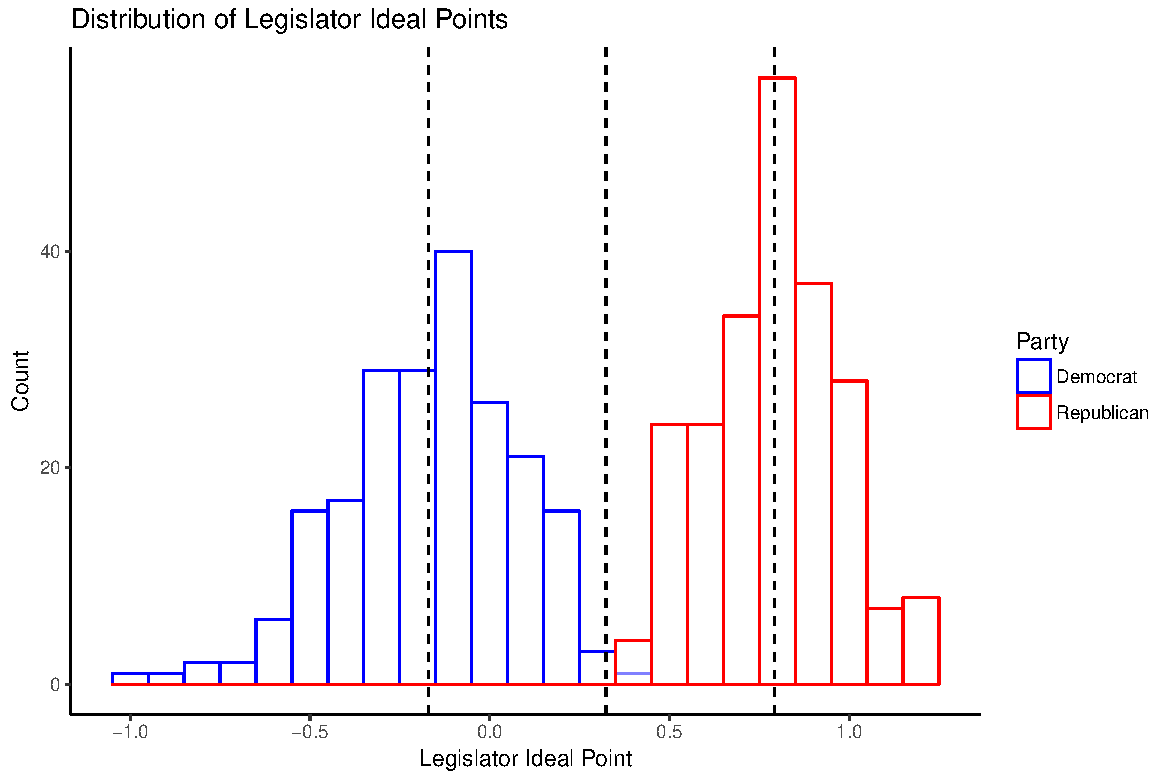
\includegraphics[width=.33\textwidth]{/Users/dsimp/GitHub/Clinton(2006)Rep/drafts/histogram-1} &
    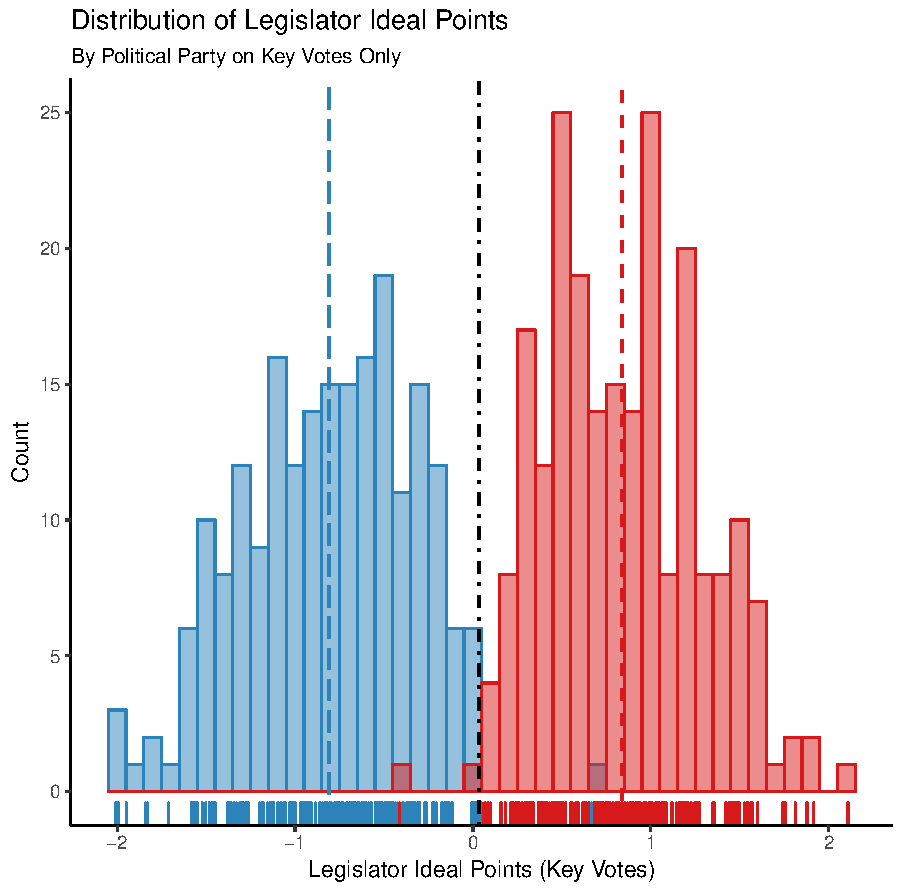
\includegraphics[width=.33\textwidth]{/Users/dsimp/GitHub/Clinton(2006)Rep/drafts/histogram-2} &
    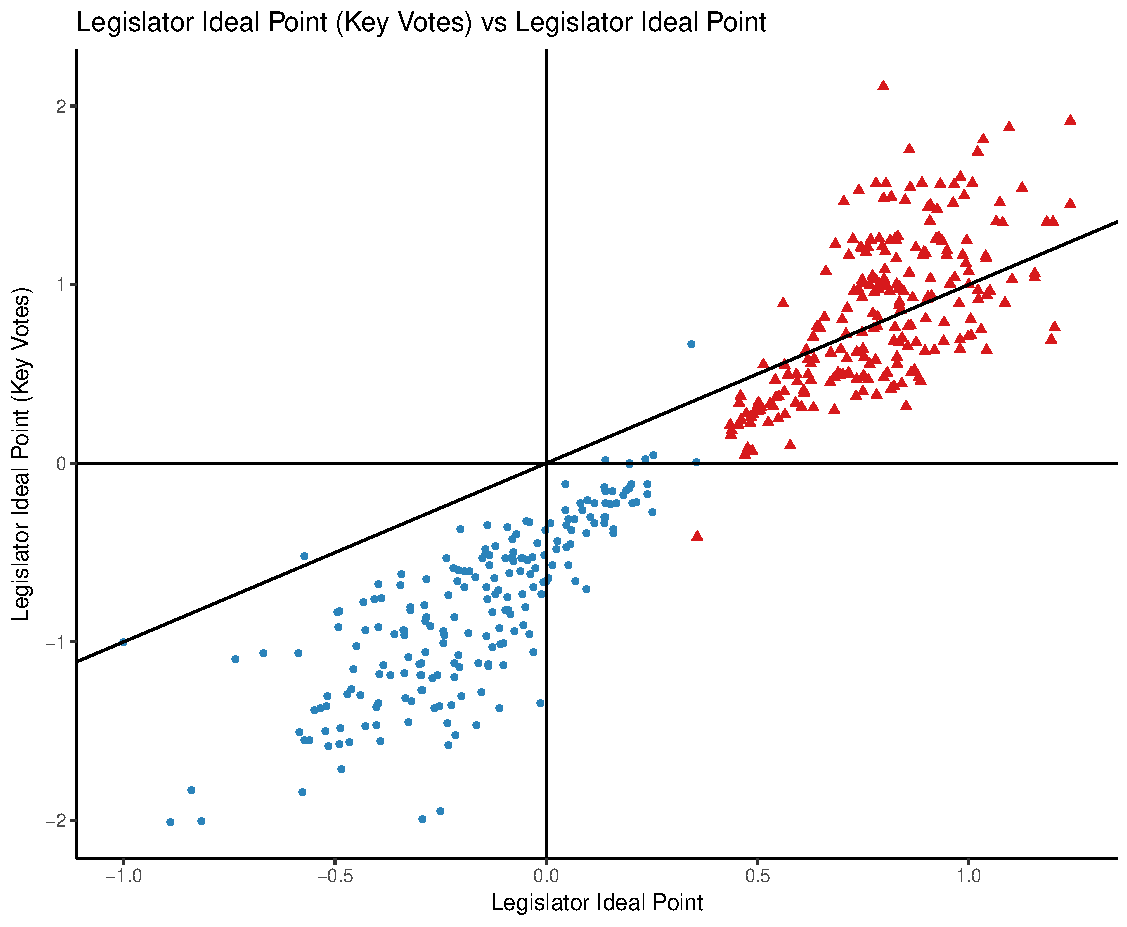
\includegraphics[width=.33\textwidth]{/Users/dsimp/GitHub/Clinton(2006)Rep/drafts/histo_change} \\
     & &  \\
    \small (D) District Mean Ideology &
    \small (E) Same-Party Mean Ideology &
    \small (F) Non-Same-Party Mean Ideology  \\
	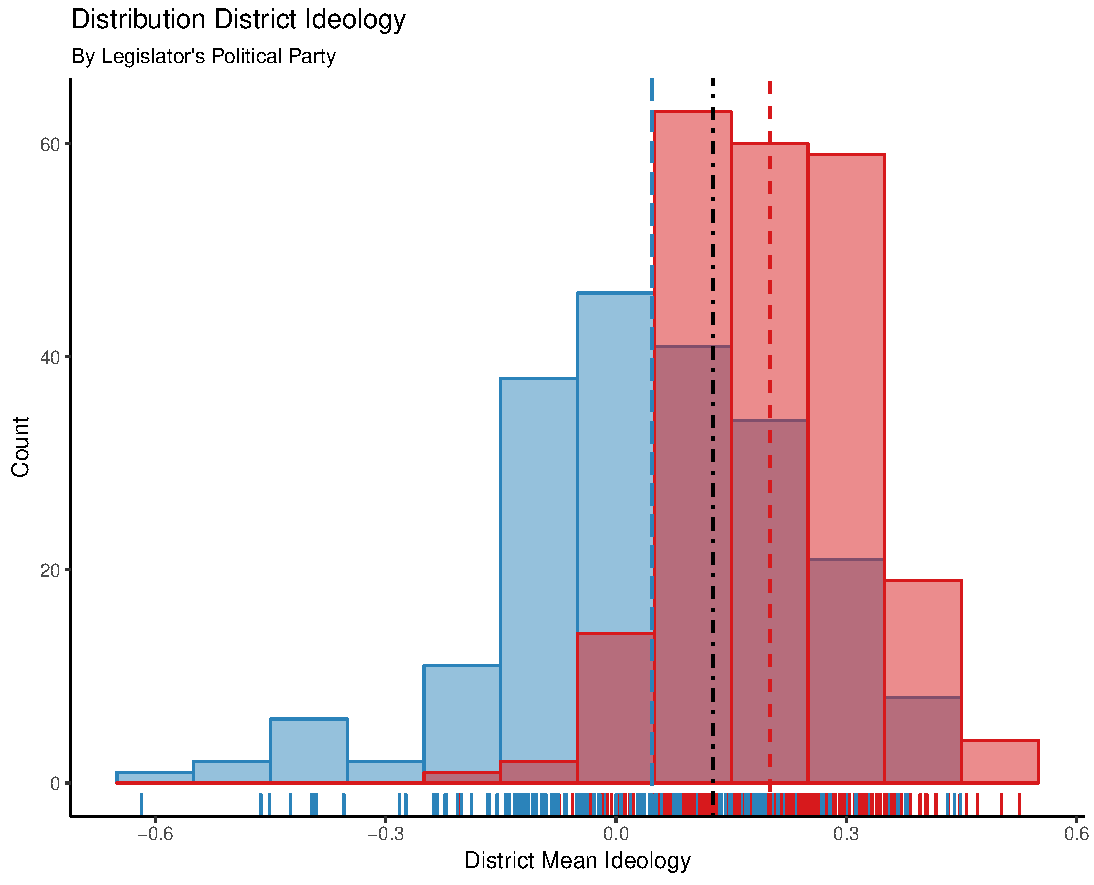
\includegraphics[width=.33\textwidth]{/Users/dsimp/GitHub/Clinton(2006)Rep/drafts/histogram-3} &
    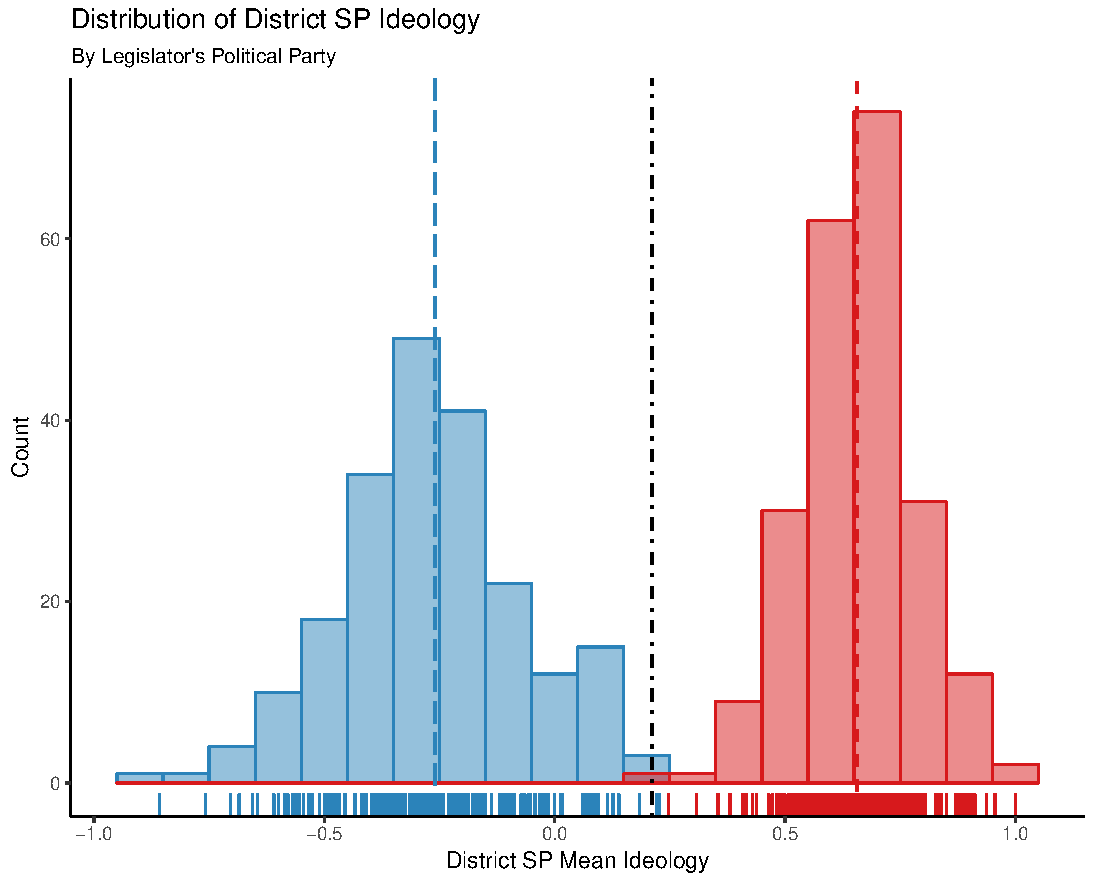
\includegraphics[width=.33\textwidth]{/Users/dsimp/GitHub/Clinton(2006)Rep/drafts/histogram-4} &
    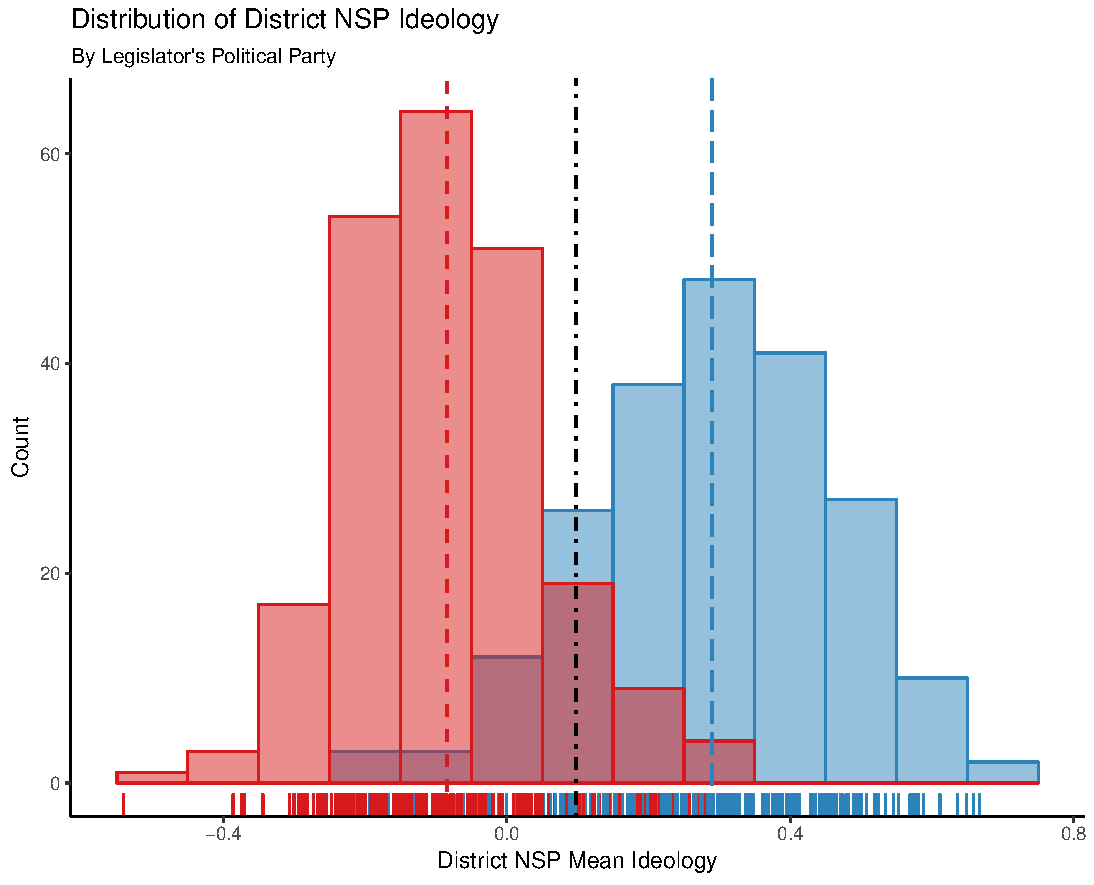
\includegraphics[width=.33\textwidth]{/Users/dsimp/GitHub/Clinton(2006)Rep/drafts/histogram-5} \\
      & &  \\
    \small (G) Opposite Party Mean Ideology&
    \small (H) Independent Mean Ideology&
    \small (I) Opposite Party vs Independent  \\
    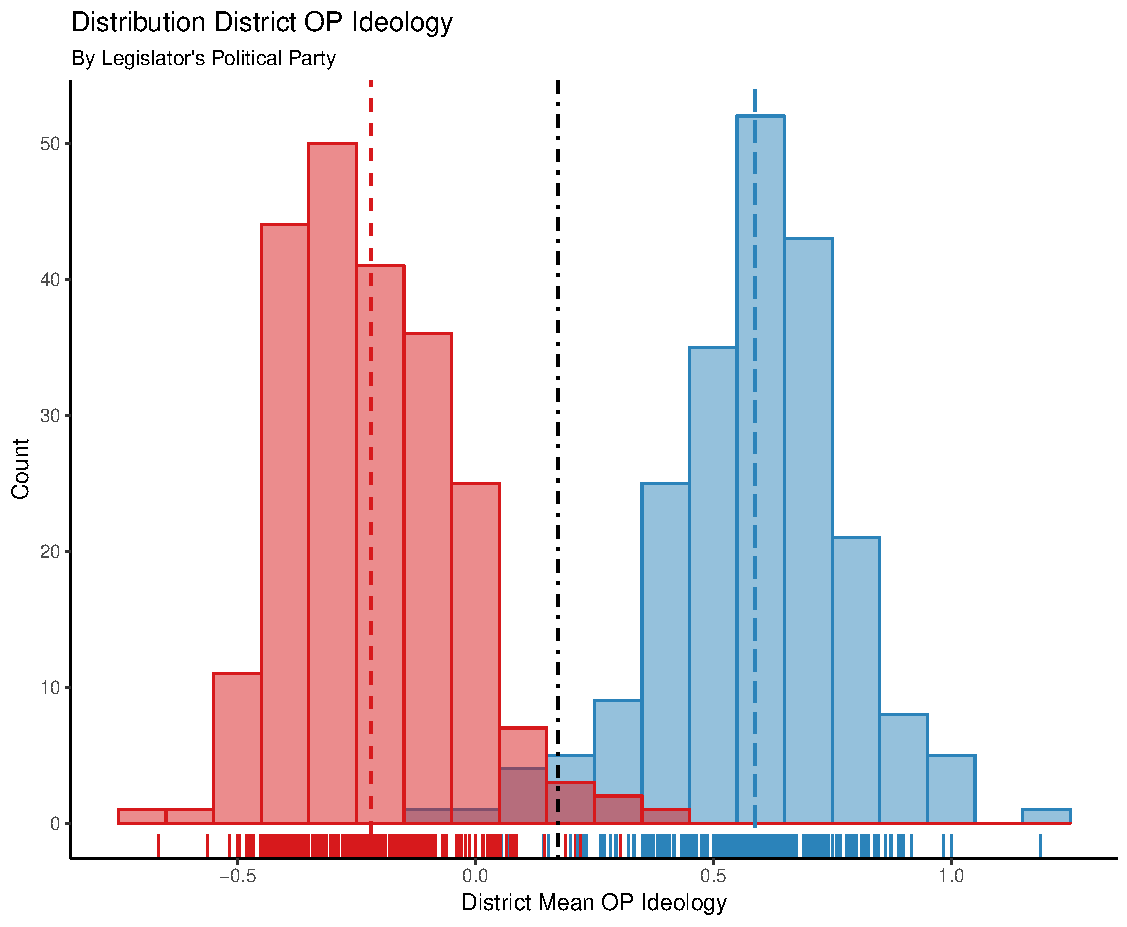
\includegraphics[width=.33\textwidth]{/Users/dsimp/GitHub/Clinton(2006)Rep/drafts/histogram-6} &
    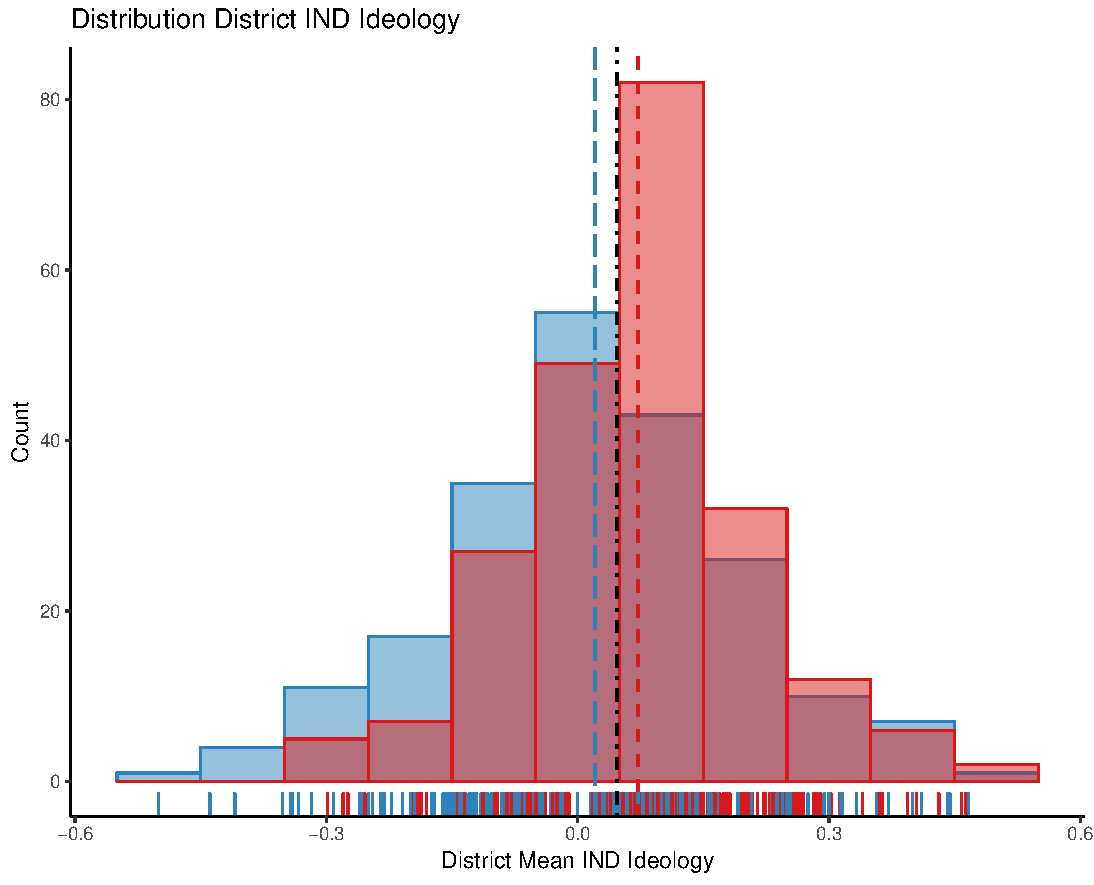
\includegraphics[width=.33\textwidth]{/Users/dsimp/GitHub/Clinton(2006)Rep/drafts/histogram-7} &
    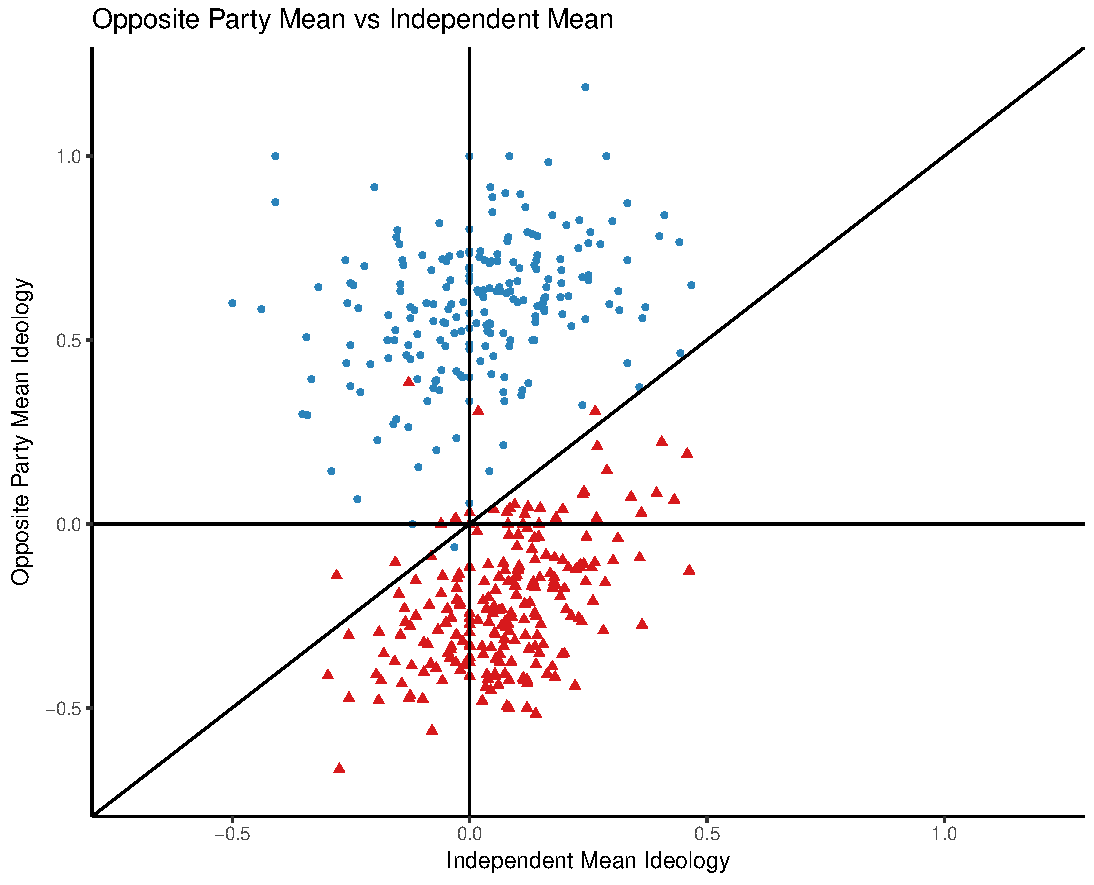
\includegraphics[width=.33\textwidth]{/Users/dsimp/GitHub/Clinton(2006)Rep/drafts/histo_diff} \\
       & &  \\
  \end{tabular}
    %}   
 \end{centering}\\
  \textbf{Note:} The histograms illustrate the distribution of legislator ideal points and sub-district constituency mean ideology grouped by legislator party. Plot (C) shows the change in district district ideal point when key votes are used instead of all votes. Points above (below) the 45-degree line are more conservative (liberal) when key votes are used. Plot (I) compares district independent mean ideology to district opposite party mean ideology. 
\end{figure}

\newpage

\begin{figure}[!htbp]
\caption{Legislator Ideal Points and District Ideology Means}
\begin{centering}
%\centering
%\fbox{
  \begin{tabular}{@{}ccc@{}}
	% & & \\  	
  	\small (A) Ideal Point &
    \small (B) Ideal Point &
    \small (C) Ideal Point  \\
    \small vs District Ideology & 
    \small vs Same-Party Ideology &
    \small vs Non-Same-Party Ideology \\
    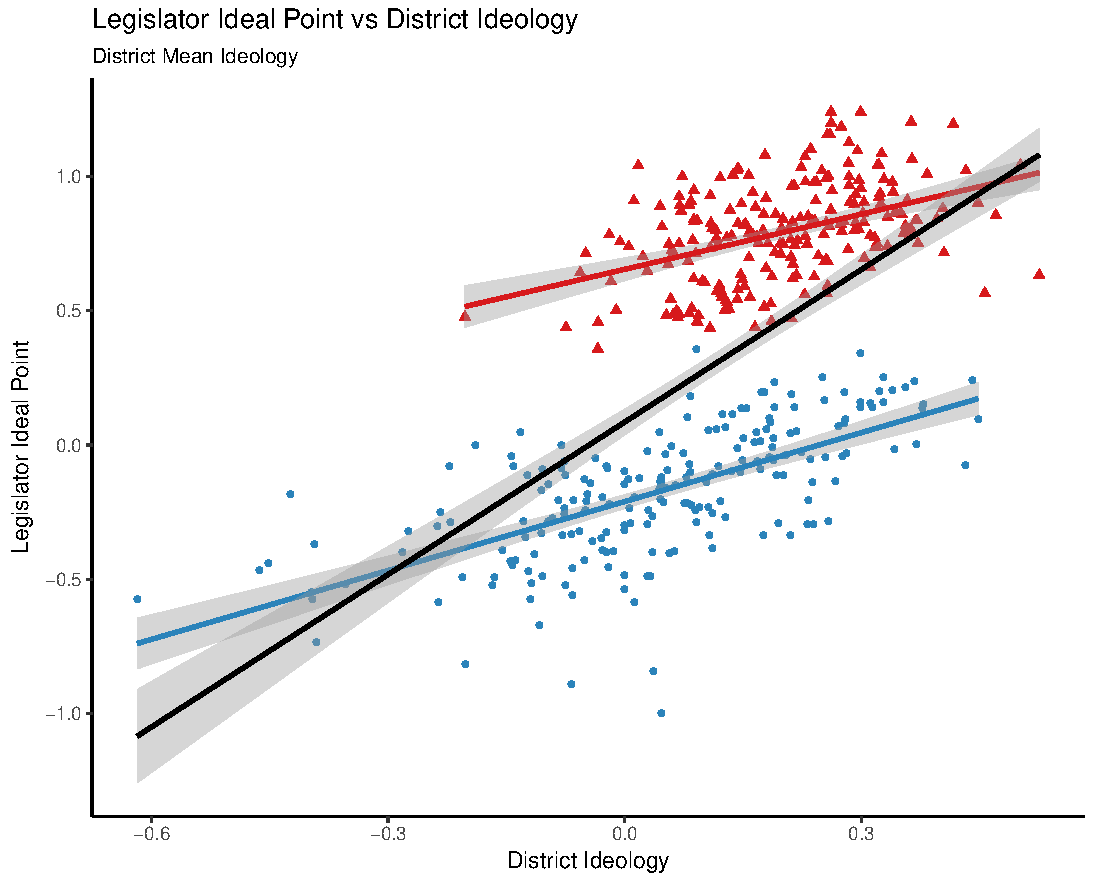
\includegraphics[width=.30\textwidth]{/Users/dsimp/GitHub/Clinton(2006)Rep/drafts/plot1-1.pdf} &
    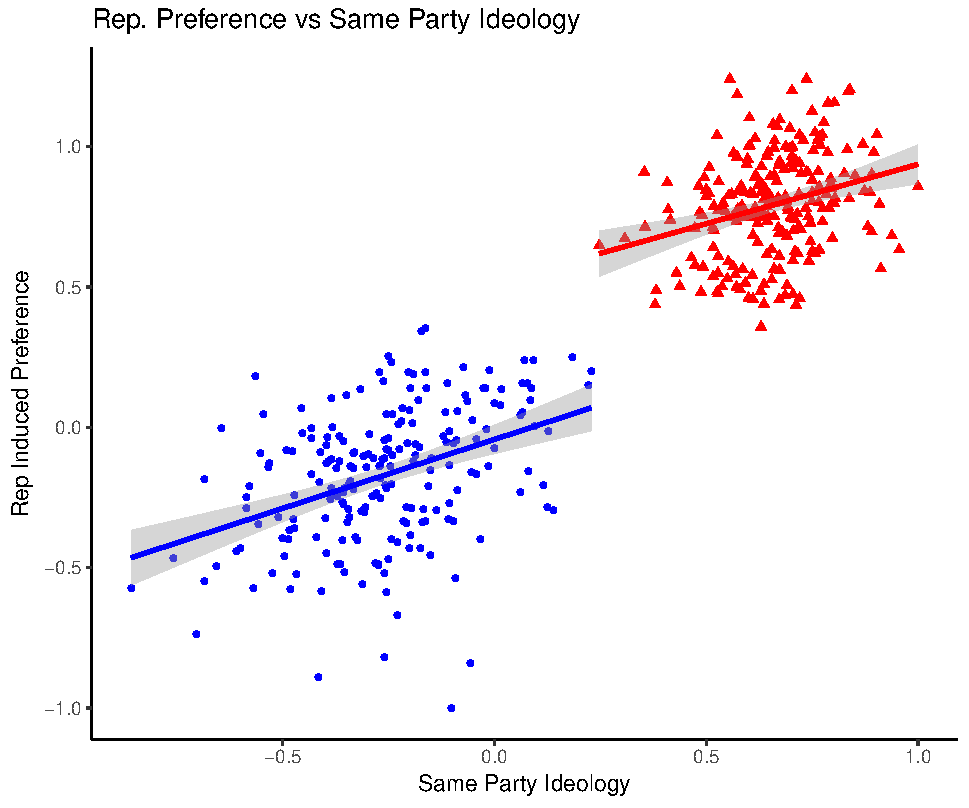
\includegraphics[width=.30\textwidth]{/Users/dsimp/GitHub/Clinton(2006)Rep/drafts/plot1-2.pdf} &
    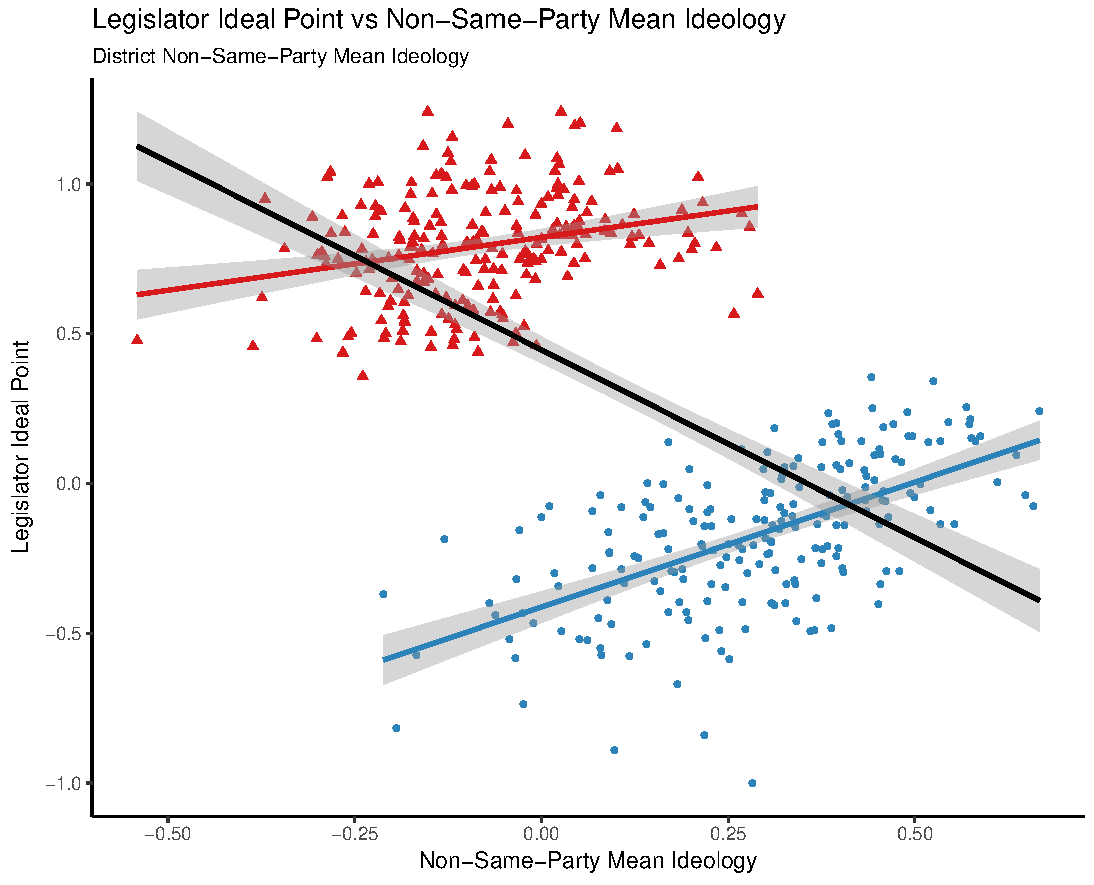
\includegraphics[width=.30\textwidth]{/Users/dsimp/GitHub/Clinton(2006)Rep/drafts/plot1-3.pdf} \\
    % & & \\
    \small (D) Ideal Point & 
    \small (E) Ideal Point & 
    \small (F) Same-Party Ideology  \\
    \small vs Opposite Party Ideology  & 
    \small vs Independent Ideology  & 
    \small vs District Ideology \\
    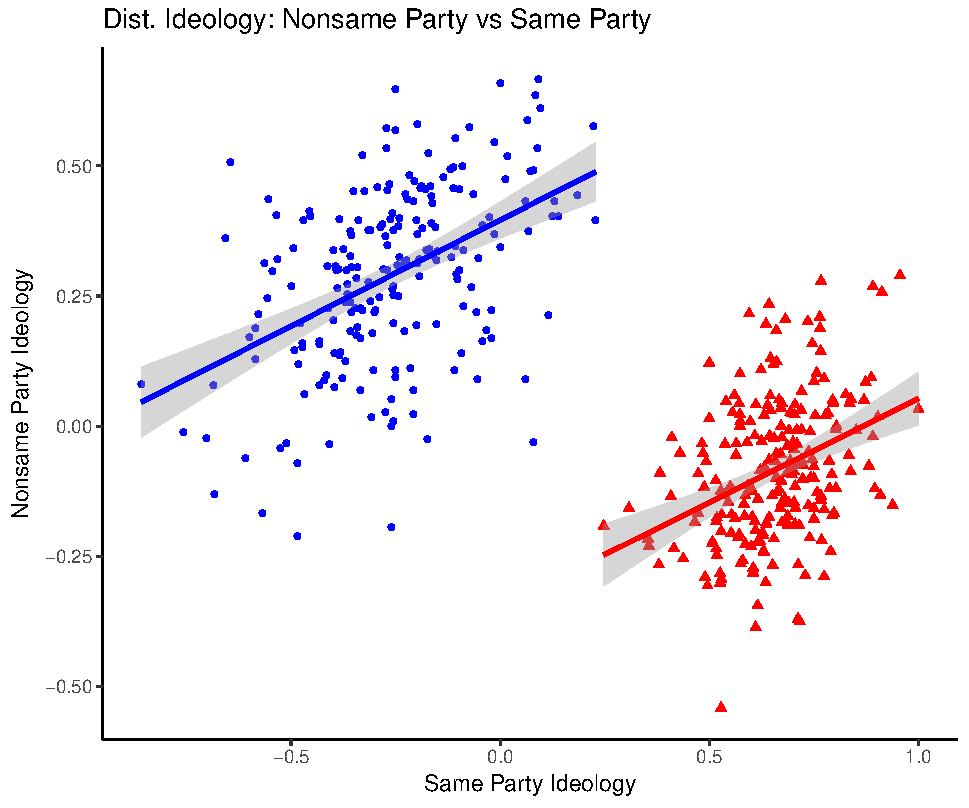
\includegraphics[width=.30\textwidth]{/Users/dsimp/GitHub/Clinton(2006)Rep/drafts/plot1-4.pdf} &
    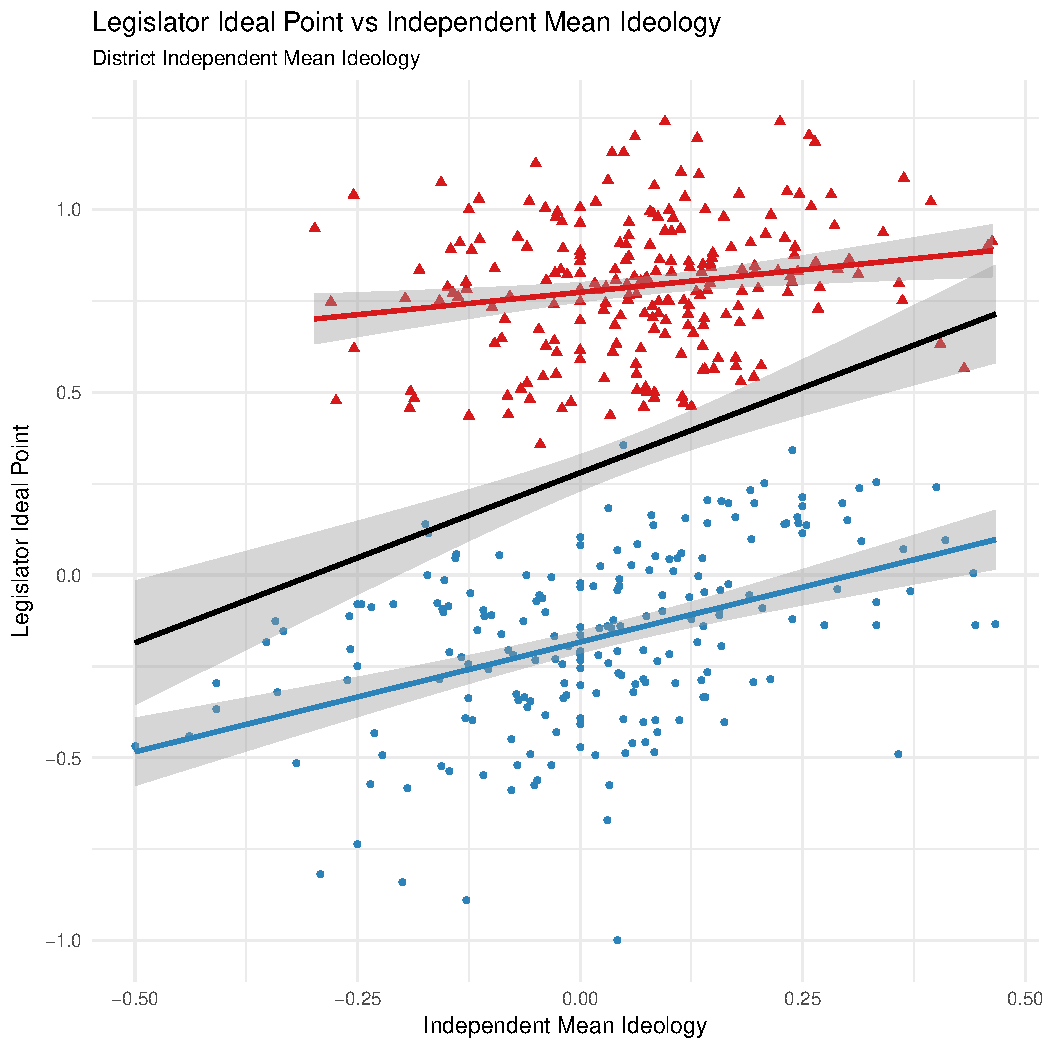
\includegraphics[width=.30\textwidth]{/Users/dsimp/GitHub/Clinton(2006)Rep/drafts/plot1-5.pdf} &
    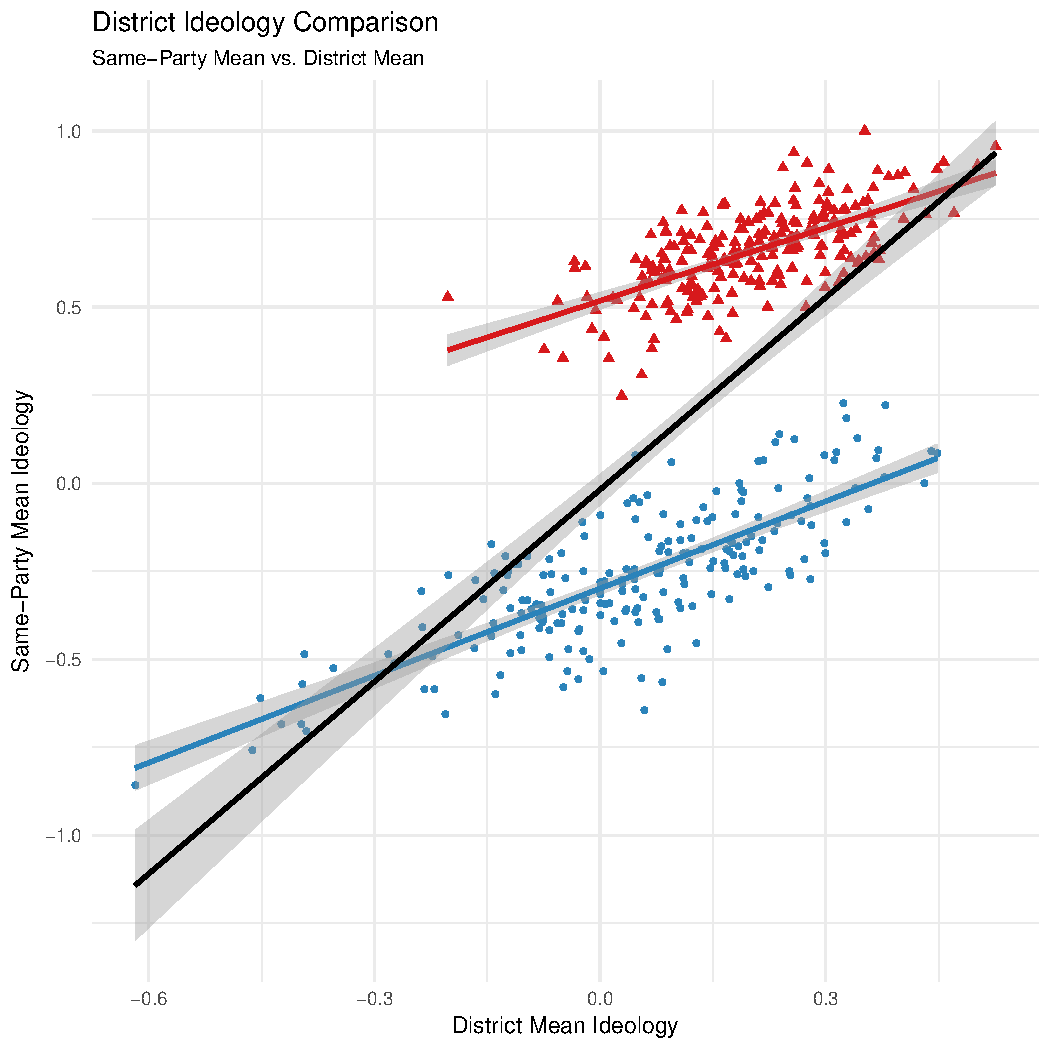
\includegraphics[width=.30\textwidth]{/Users/dsimp/GitHub/Clinton(2006)Rep/drafts/plot1-6.pdf} \\
    % &  &\\
    \small (G) Non-Same-Party Ideology & 
    \small (H) Opposite Party Ideology & 
    \small (I) Independent Ideology  \\
    \small vs District Ideology  & 
    \small vs District Ideology  & 
    \small vs District Ideology \\
    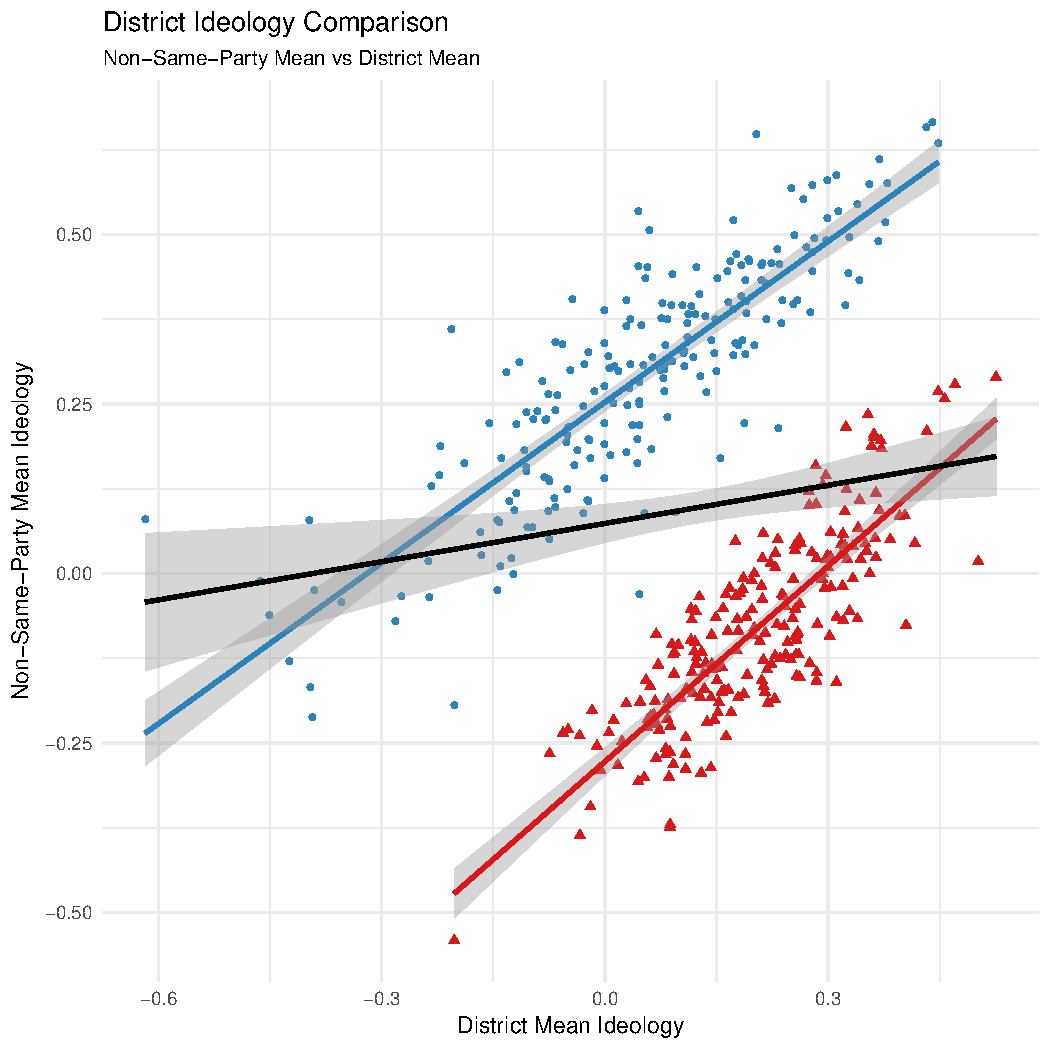
\includegraphics[width=.30\textwidth]{/Users/dsimp/GitHub/Clinton(2006)Rep/drafts/plot1-7.pdf} &
    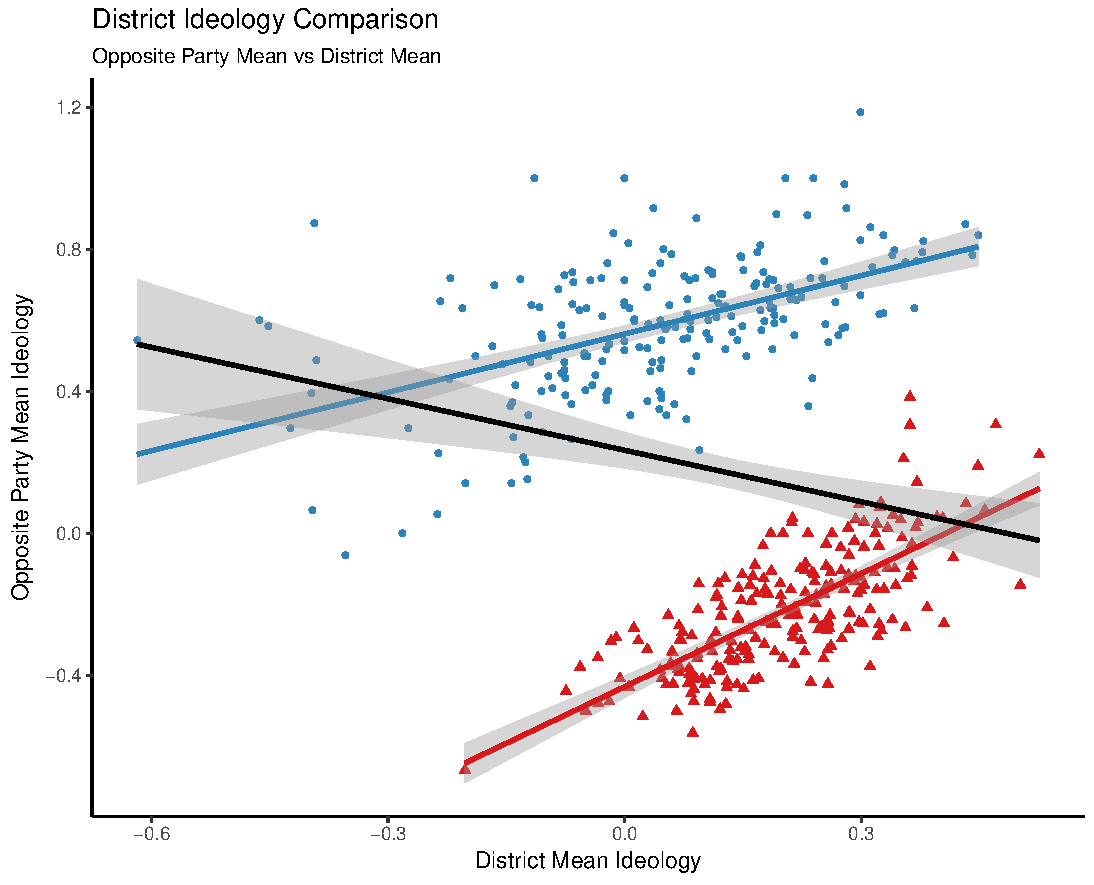
\includegraphics[width=.30\textwidth]{/Users/dsimp/GitHub/Clinton(2006)Rep/drafts/plot1-8.pdf} &
    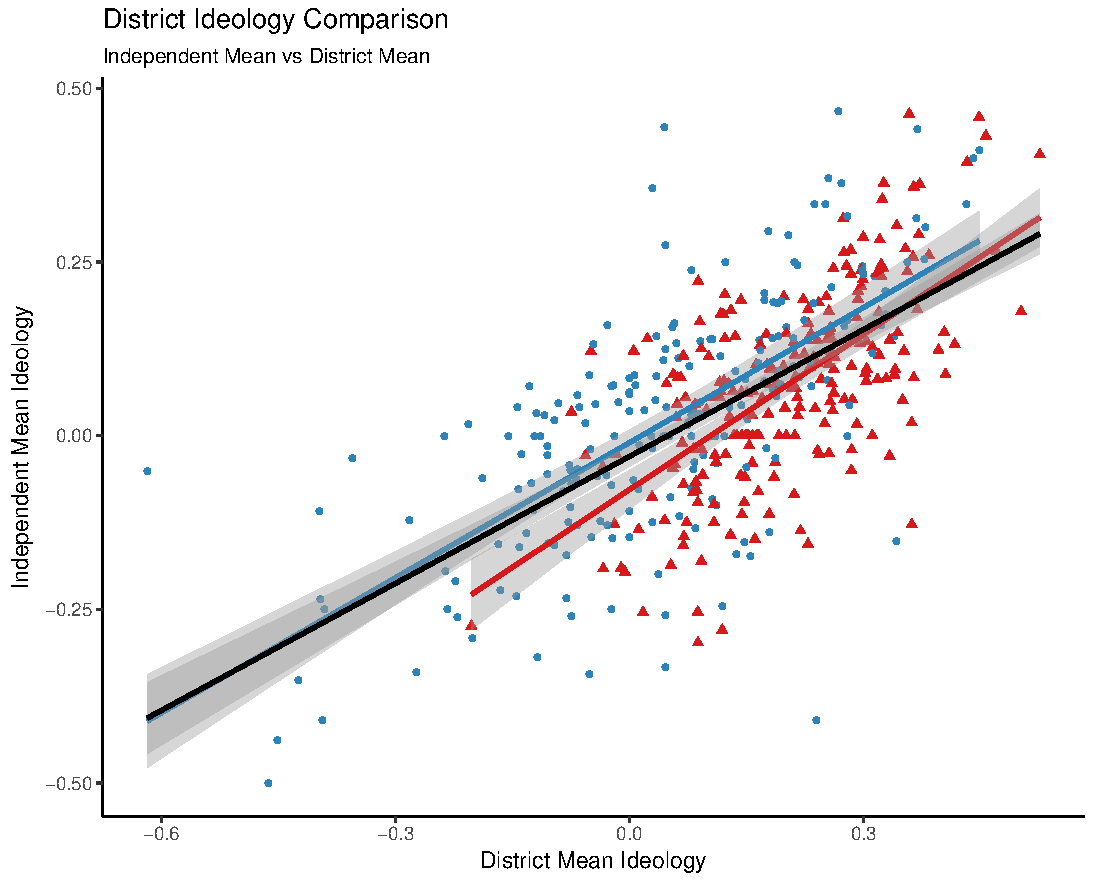
\includegraphics[width=.30\textwidth]{/Users/dsimp/GitHub/Clinton(2006)Rep/drafts/plot1-9.pdf} \\
    % &  &\\
    \small (J) Non-Same-Party Ideology & 
    \small (K) Opposite Party Ideology & 
    \small (L) Independent Ideology  \\
    \small vs Same-Party Ideology  & 
    \small vs Same-Party Ideology  & 
    \small vs Same-Party Ideology \\
    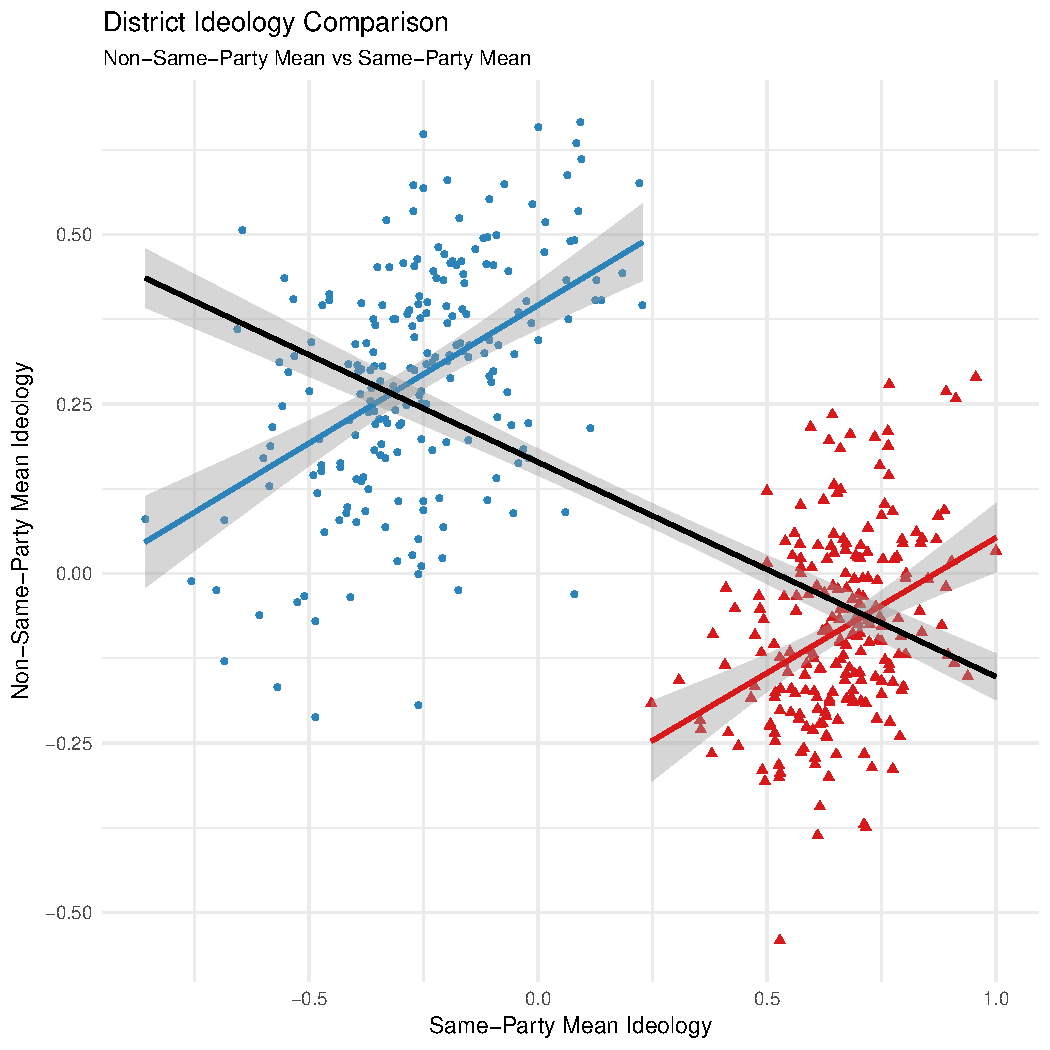
\includegraphics[width=.30\textwidth]{/Users/dsimp/GitHub/Clinton(2006)Rep/drafts/plot1-10.pdf} &
    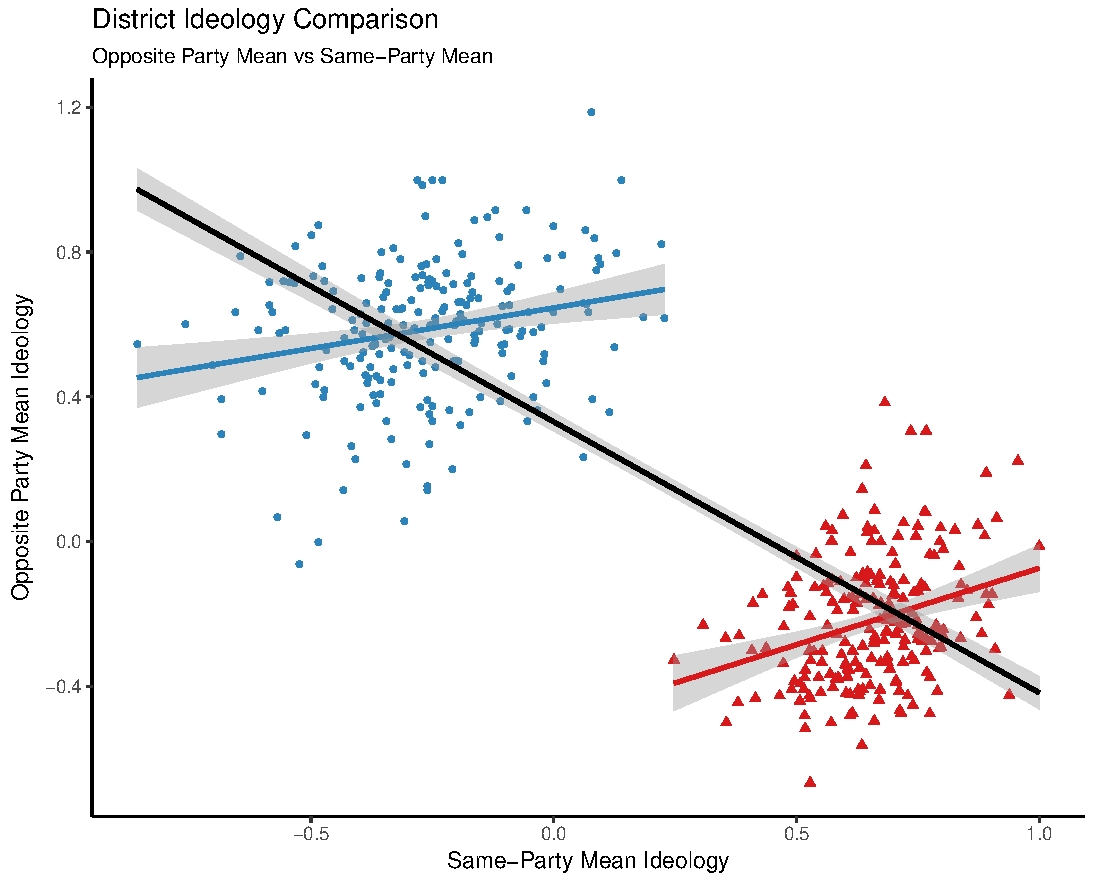
\includegraphics[width=.30\textwidth]{/Users/dsimp/GitHub/Clinton(2006)Rep/drafts/plot1-11.pdf} &
    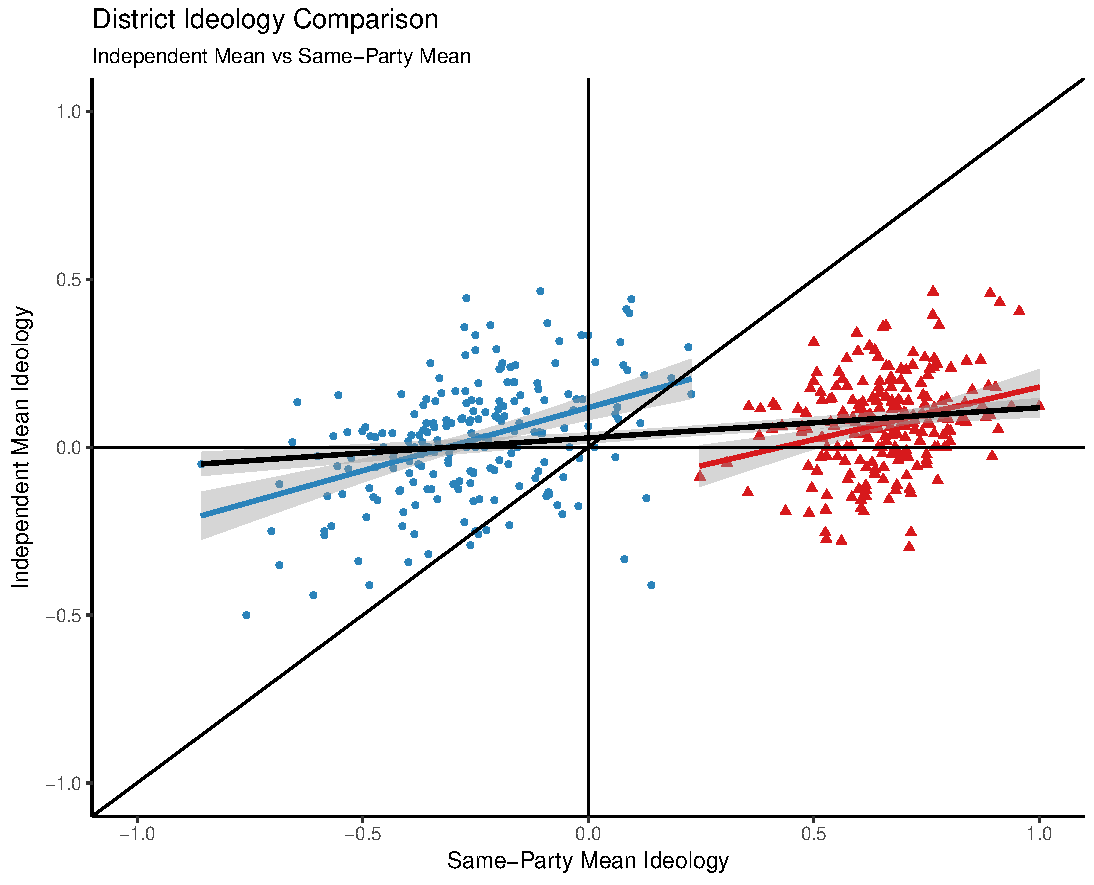
\includegraphics[width=.30\textwidth]{/Users/dsimp/GitHub/Clinton(2006)Rep/drafts/plot1-12.pdf} \\
  \end{tabular}
    %}   
 \end{centering}
  \textbf{Note:} In each panel, districts represented by a Republican (Democrat) are plotted with a triangle (circle). A bivariate trendline is added for the overall comparison and bivariate trendlines are added for comparison within districts represented by Republicans and Democrats.
\end{figure}

\newpage



\section{Initial Findings} 

\subsection{Interaction Terms}
The main empirical issue in \citep{Clinton2006} is that each model with interaction terms omits the constitutive terms necessary for determining the relationship between sub-district ideology and legislator ideal point. \cite{Brambor2006} argue that there is almost never a valid reason to omit constitutive variables when a model includes interaction terms. Observe the below equation (1) which appears in Clinton's Table 1. The model regresses legislator ideal points ($y_i$) on weighted sub-district level weighted average ideology scores. The terms $w_{SP_i}$ and $w_{NSP_i}$ respectively weight same-party average ideology ($\bar{z}_{SP_i}$) and non-same-party average ideology ($\bar{z}_{NSP_i}$) by the share of group members sampled in each district. As such, the weights in equation (1) are defined $w_{SP_i} = \frac{n_i^{SP}}{n_i}$ and $w_{NSP_i} =  \frac{n_i^{SP}}{n_i}$. The term $I_{GOP}$ is a party indicator variable. 

\begin{equation}
y_i  = \beta_0 + \beta_1 w_{SP_i} \bar{z}_{SP_i} + \beta_2 w_{NSP_i} \bar{z}_{NSP_i} + \gamma I_{GOP} + \varepsilon_i
\end{equation}
This specification is incorrect and yields biased coefficient values and underestimated coefficient variance values. The correct specification of model (1) should include $w_{SP_i}$, $w_{NSP_i}$, $\bar{z}_{SP_i}$, $\bar{z}_{SP_i}$ each as individual independent variables in addition to their interaction. As such, the correctly specified model is given in the below equation (2).
\begin{equation}
\begin{array}{ccc}
y_i & = & \alpha_0 + \alpha_1 w_{SP_i} \bar{z}_{SP_i} + \alpha_2 w_{NSP_i} \bar{z}_{NSP_i} + \alpha_3 \bar{z}_{SP_i}~~~~~~~~~\\ 
& & ~~+ \alpha_4 \bar{z}_{NSP_i} + \alpha_5 w_{SP_i} + \alpha_6 w_{NSP_i} + \lambda I_{GOP} + \epsilon_i
\end{array}
\end{equation}
Equation (1) implies that one can estimate the unconditional marginal effect of weighted group ideology (i.e. $\beta_1$ for the single term $\big( \frac{n_i^{SP}}{n_i} \bar{z}_{SP_i}\big)$ and that neither the weights nor sub-district group ideologies have an effect on legislator ideal point. That is, equation (1) effectively assumes that $\alpha_3$, $\alpha_4$, $\alpha_5$, and $\alpha_6$ from equation (2) are all zero. Empirically, this is incorrect. Intuitively, one should expect group size $w_{j\in \{SP,NSP\}_i}$ and group ideology $\bar{z}_{j\in \{SP,NSP\}_i}$ to individually influence legislator behavior. One should also expect the impact of group share (ideology) to change as group ideology (share) changes.

Empirically, the marginal effect of group share (ideology) is given by the derivative of legislator ideal point with respect to share (ideology). For example in equation (2), the relationship between legislator ideal point and same-party ideology is: 
$$\frac{\partial y_i}{\partial \bar{z}_{SP_i}}= \alpha_1 w_{SP_i} + \alpha_3$$
The coefficient $\alpha_3$ captures the portion of the slope $\frac{\partial y}{\partial \bar{z}_{SP_i}}$ (the relationship between ideal point and same-party ideology) that is constant across all districts regardless of the district share of same-party constituents. The terms $\alpha_1 w_{SP_i}$ captures how the slope $\frac{\partial y}{\partial \bar{z}_{SP_i}}$ changes as the district share of same-party constituents increases. Therefore equation (2) is underspecified and the estimates of $\beta_1$ and $\beta_2$ will be biased. For example, the coefficient $\beta_1$ on weighted same-party ideology in equation (1) is capturing $\alpha_1$, $\alpha_3$ and $\alpha_5$ from equation (4).

Additionally, it is important to note that the use of interaction terms implies that a second calculation is necessary to determine the standard errors for the marginal effects of group share or group ideology. One cannot simply rely on usually reported coefficient values and standard errors to determine statistical significance of a variable that is included in an interaction term. Rather, it is necessary to directly calculate the variance term. For example, consider the marginal effect of same-party ideology. The variance is given as:  $var(\frac{\partial y}{\partial \bar{z}_{SP_i}})$. That is $var(\frac{\partial y}{\partial \bar{z}_{SP_i}}) = var(\alpha_1 w_{SP_i} + \alpha_4)$. Therefore, the standard error term for $\frac{\partial y}{\partial \bar{z}_{SP_i}}$ is given by:
$$\hat{\sigma}_{\partial y_i / \partial \bar{z}_{SP_i}} = \sqrt{w_{SP}^2var(\hat{\alpha}_1)+var(\hat{\alpha}_3)+2w_{SP}cov(\hat{\alpha}_1\hat{\alpha}_3)}$$

The below Table 1 provides the regression results for models 1 and 2. Model 1 is a replication of Clinton (2006)'s Table 1 Model 2. The Model 1 results replicated here are identical to those found in Clinton (2006). Model 2 is the correctly specified model with each of the interaction terms. However, Percent Same-Party and Percent Non-Same Party are perfectly multicolinear by construction. Therefore, Percent Non-Same-Party is omitted. Under this specification, one cannot estimate the marginal effect Percent Non-Same Party; however, Model 3 omits the constant term and allows for estimation of the marginal effect of Percent Non-Same Party.

$$Insert ~ Explanation~Of~Results~Here$$

Insert chart showing the difference of the regression predictions for the two models using same-party ideology and non-same party ideology. Include in the new figure 2.

Figure 3 provides an illustration of the marginal effects of group share and group ideology for both same- and non-same-party.

$$Insert ~ Explanation~Of~Results~Here$$

\input{/Users/dsimp/GitHub/Clinton(2006)Rep/drafts/table2.txt}




\begin{figure}[!htbp]
\caption{Representative Ideal Points and District Ideology (Reproduced)}
\begin{centering}
%\centering
%\fbox{
  \begin{tabular}{@{}cc@{}}
	 & \\  	
  	\small (A) Marginal Effect of Same-Party Ideology & 
    \small (B) Marginal Effect of Percent Same-Party  \\
    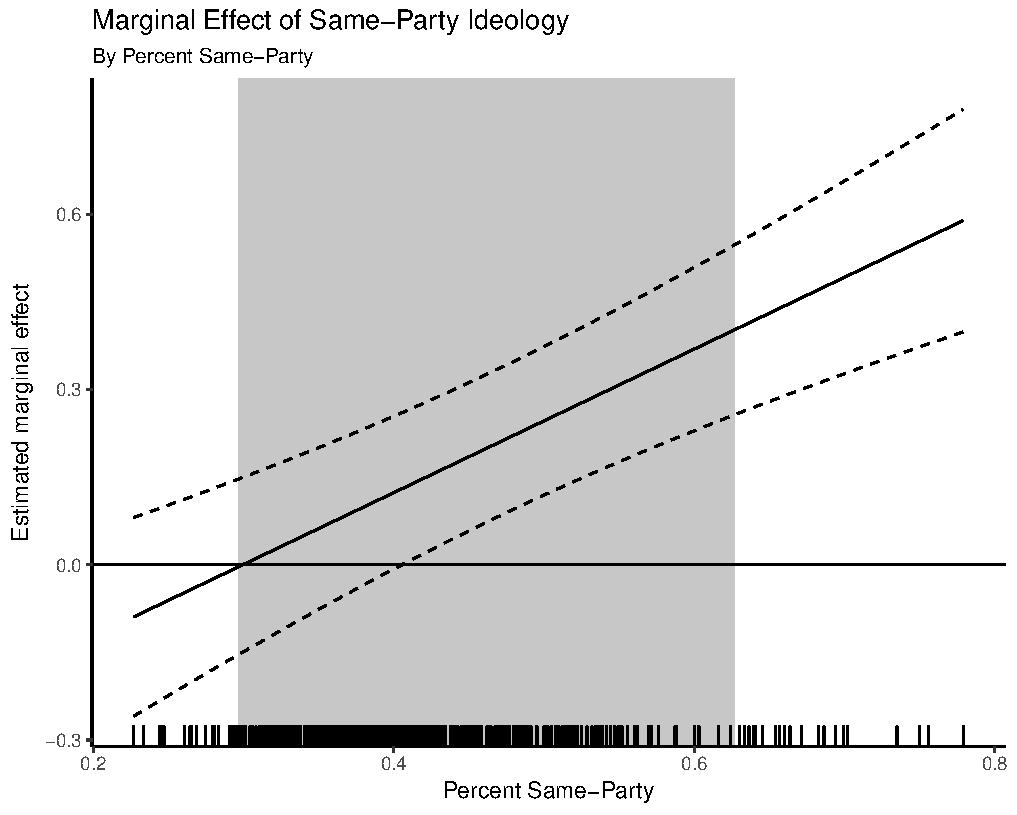
\includegraphics[width=.45\textwidth]{/Users/dsimp/GitHub/Clinton(2006)Rep/drafts/me-1.pdf} &
    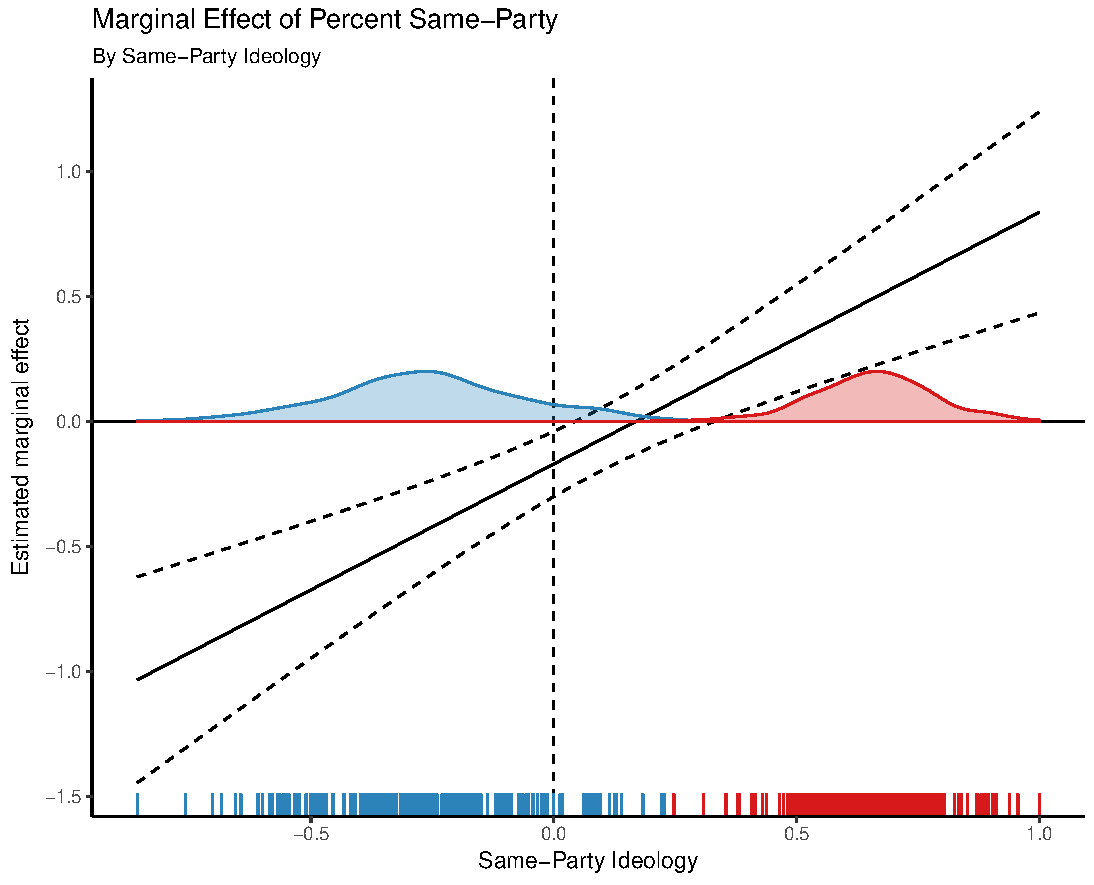
\includegraphics[width=.45\textwidth]{/Users/dsimp/GitHub/Clinton(2006)Rep/drafts/me-2.pdf} \\
     & \\
    \small (C) Marginal Effect of Non-Same-Party Ideology & 
    \small (D) Marginal Effect of Percent Non-Same-Party \\
    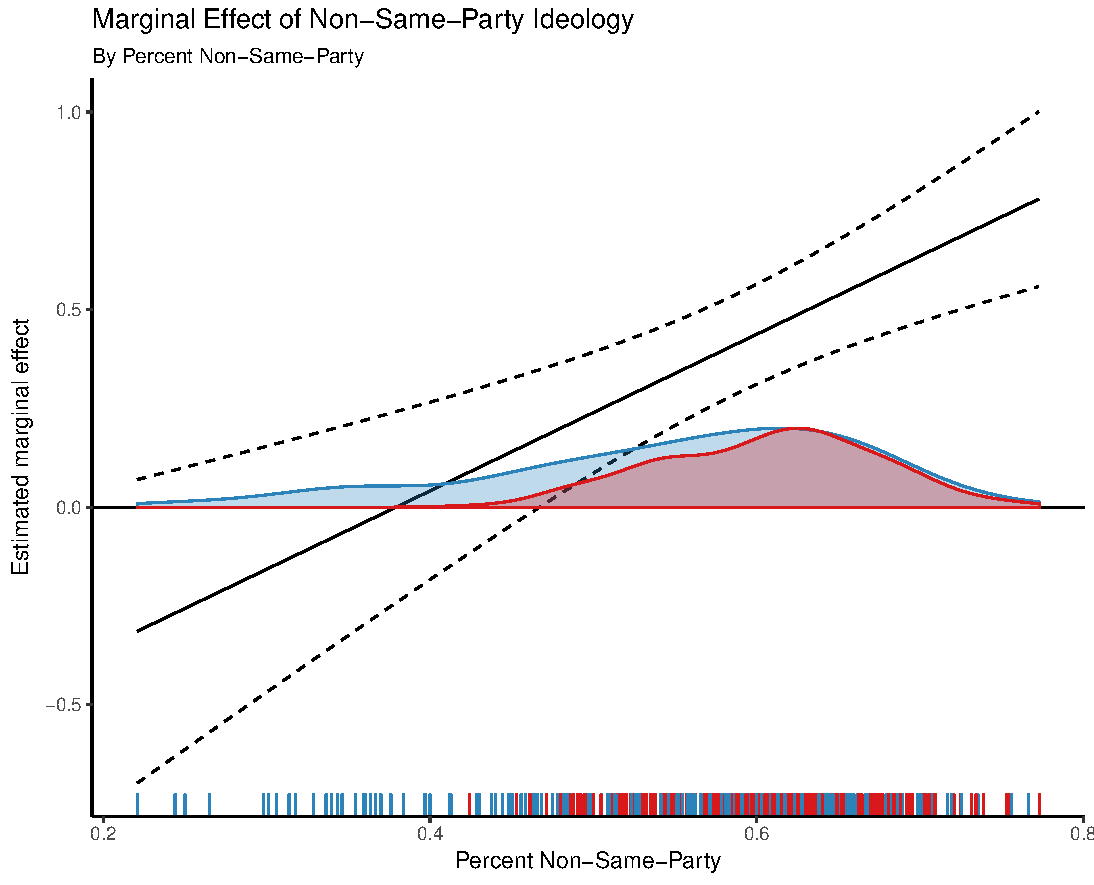
\includegraphics[width=.45\textwidth]{/Users/dsimp/GitHub/Clinton(2006)Rep/drafts/me-3.pdf} &
    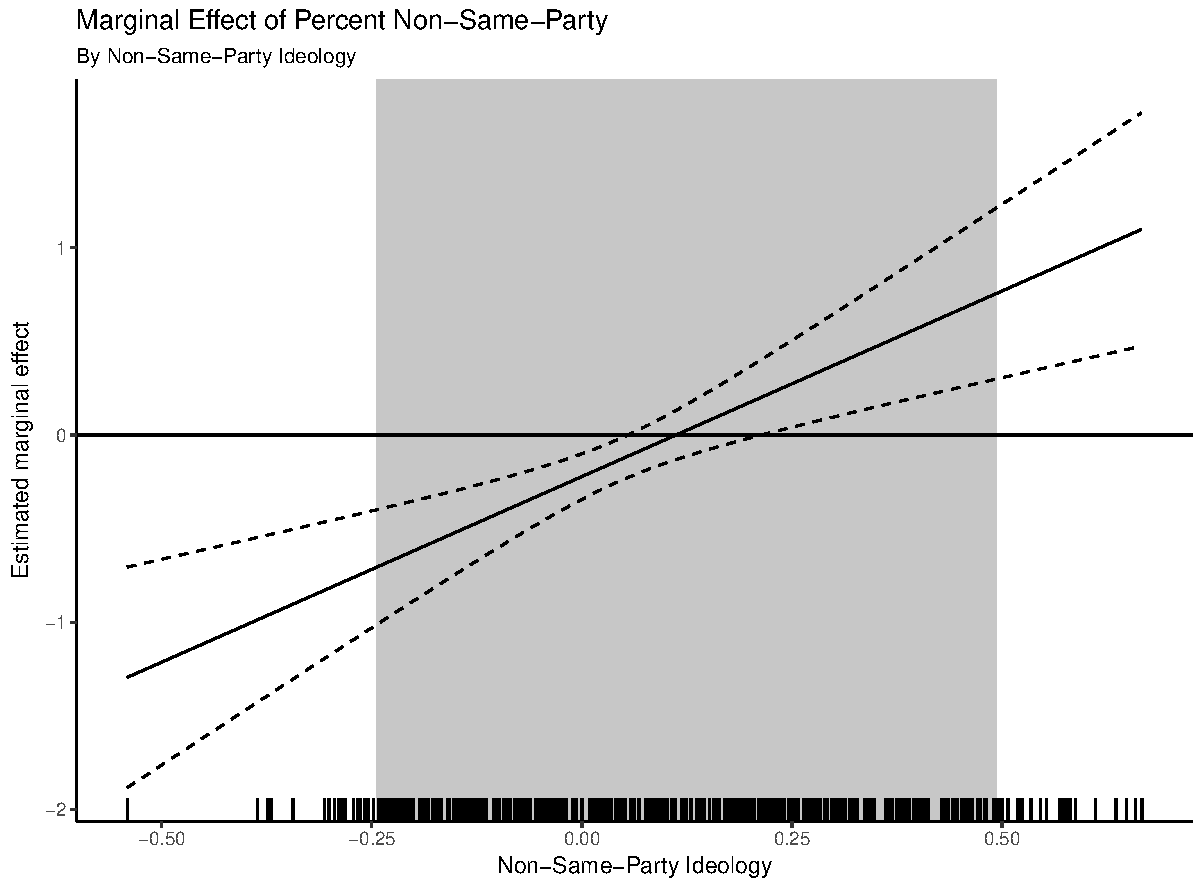
\includegraphics[width=.45\textwidth]{/Users/dsimp/GitHub/Clinton(2006)Rep/drafts/me-4.pdf} \\
     &  \\
  \end{tabular}
    %}   
 \end{centering}
  \textbf{Note:} Each panel plots the respective marginal effect of the constitutive terms of the interaction variables in Table 1 Model 3.
\end{figure}

Clinton (2006) includes an errors in variable regression in the analysis following the practice of Gerald C. Wright, Robert S. Erikson and John P. McIver, and Fuller (1987).

\newpage

\subsection{Transformations and Interpretation}
A second, those less problematic, issue in the \cite{Clinton2006} analysis is tha

\newpage


\subsection{Ideology Scores}
To assess subconstituency influence on legislator behavior, \cite{Clinton2006} decomposes geographic constituency preferences into two weighted groups. The average ideology score $\bar{z}_i$ for each district $i$ is separated into the sample-population weighted same-party constituency preference $\frac{n_i^{SP}}{n_i}$ $\bar{z}_{SP_i}$ and the weighted nonsame-party constituency preference $\frac{n_i^{NSP}}{n_i}$ $\bar{z}_{NSP_i}$. The decomposition is shown in the below equation (3).

See equation (1):
\begin{equation}
\bar{z}_i = \bigg( \frac{n_i^{sp}}{n_i} \bigg) \bar{z}_{SP_i} + \bigg( \frac{n_i^{SP}}{n_i} \bigg) \bar{z}_{NSP_i}
\end{equation}
As stated above and shown in equation (1), \cite{Clinton2006} regresses legislator ideal points on the district party decomposition and a party indicator variable. Equation (2) and Table 1 models 2-4 demonstrate the problems with failing to include the constitutive variables of the interaction terms. However, the decomposition into two groups pose addition specification issues if independent voters are a large share of the non-same-party constituency and if these independent voters also voted for their district's current representative. 

\textit{However, such a specification can yield biased results if independent voters who are a large share of the nonsame-party constituency - especially if many independent voters also voted for their current representative.} \textbf{Figure 1, panel (I) demonstrates this potential problem. In Democratic districts, independent voters span the range -0.50 to 0.50, yet the same district opposite party voters are on average more conservative, with most scores falling between 0 and 1.2.} Similarly, in Republican districts independent voters are more conservative, with \textbf{Insert the comparison.} As such, it should be expected that legislators are sensitive to opinions of independent voters especially \textbf{when words}.

There is reason to expect this given democratic legislators span the spectrum of district ideology scores (See the below figure X). As such, decomposing district ideology scores into weighted same-party, weighted independent voters $\frac{n_i^{I}}{n_i}$ $\bar{z}_{I_i}$, and weighted opposite-party $\frac{n_i^{OP}}{n_i}$ $\bar{z}_{OP_i}$ will address this issue. The new specification is shown in equation (3).
\begin{equation}
y_i  = \beta_0 + \beta_1 \bigg( \frac{n_i^{SP}}{n_i} \bigg) \bar{z}_{SP_i} + \beta_3 \bigg( \frac{n_i^{I}}{n_i} \bigg) \bar{z}_{I_i} + \beta_4 \bigg( \frac{n_i^{OP}}{n_i} \bigg) \bar{z}_{OP_i} + \gamma I_{GOP} + \varepsilon_i
\end{equation}

\textbf{Do a marginal effects figure for same-party and non-same party as well. This can be used to show why the findings in Clinton (2006) are wrong.}

\newpage


\input{/Users/dsimp/GitHub/Clinton(2006)Rep/drafts/table3.txt}


% 

\begin{figure}[!htbp]
\caption{Marginal Effects of Interaction Terms}
\begin{centering}
%\centering
%\fbox{
  \begin{tabular}{ccc}%{@{}ccc@{}}
	& \small \textbf{GOP Regression} & \\ 
	& & \\ 	
  	\small (A) Percent Same-Party& 
  	\small (B) Percent Opposite-Party& 
    \small (C) Percent Independent\\
    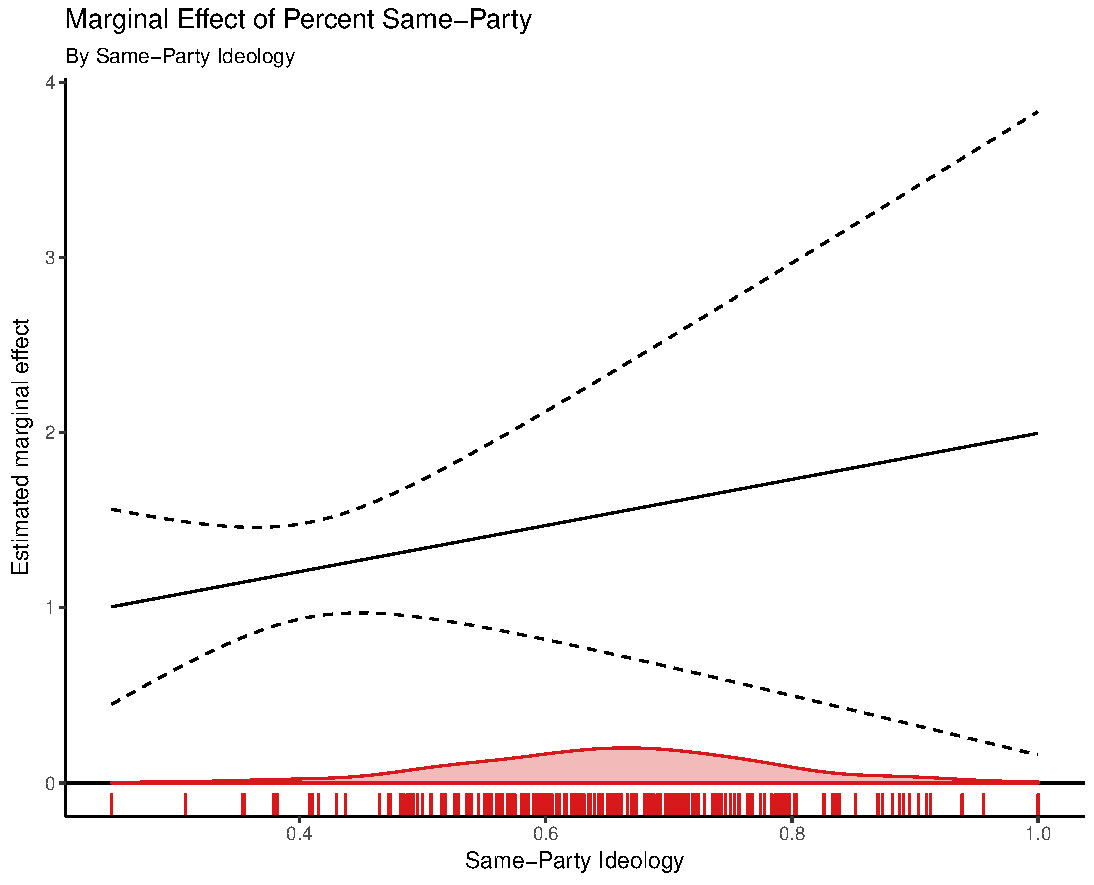
\includegraphics[width=.25\textwidth]{/Users/dsimp/GitHub/Clinton(2006)Rep/drafts/me2-1} &
    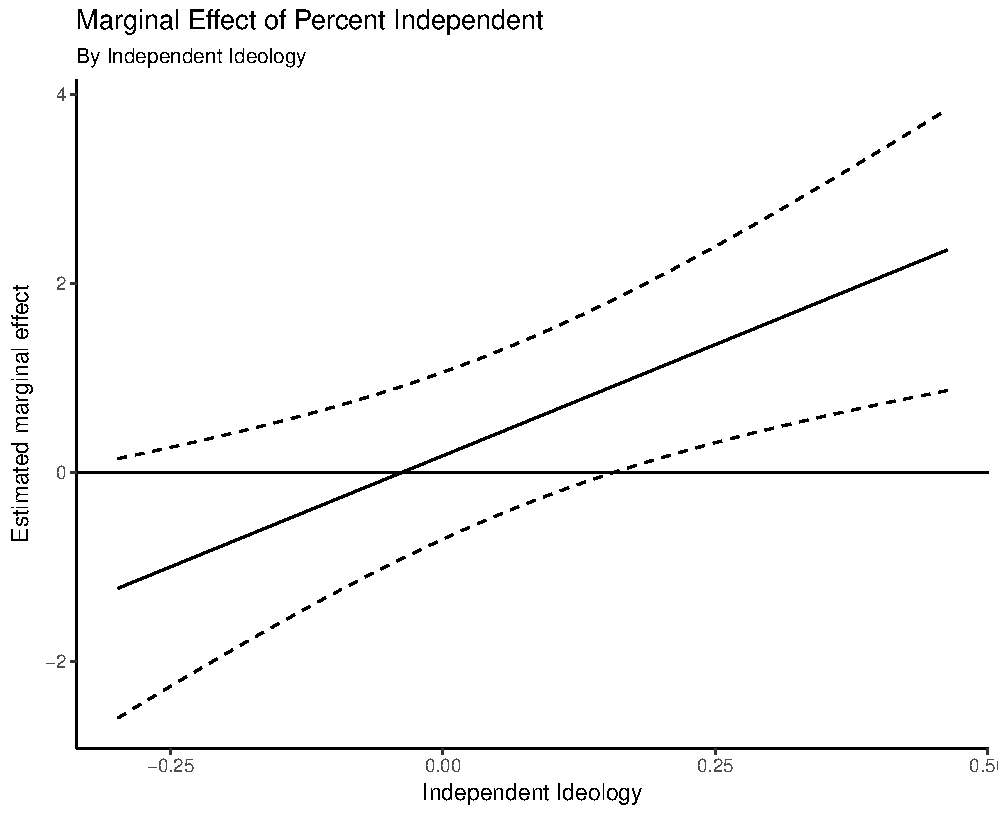
\includegraphics[width=.25\textwidth]{/Users/dsimp/GitHub/Clinton(2006)Rep/drafts/me2-3} &
    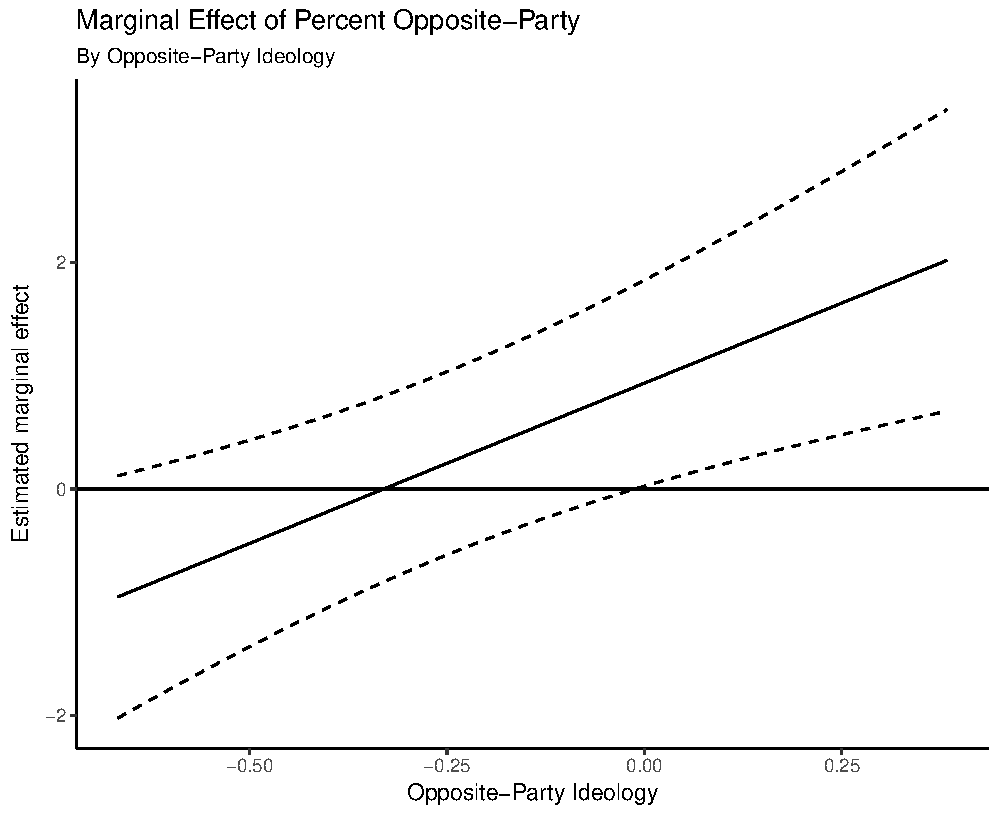
\includegraphics[width=.25\textwidth]{/Users/dsimp/GitHub/Clinton(2006)Rep/drafts/me2-5} \\
     & & \\
  	\small (D) Same-Party Ideology& 
  	\small (E) Opposite-Party Ideology& 
    \small (F) Independent Ideology\\
    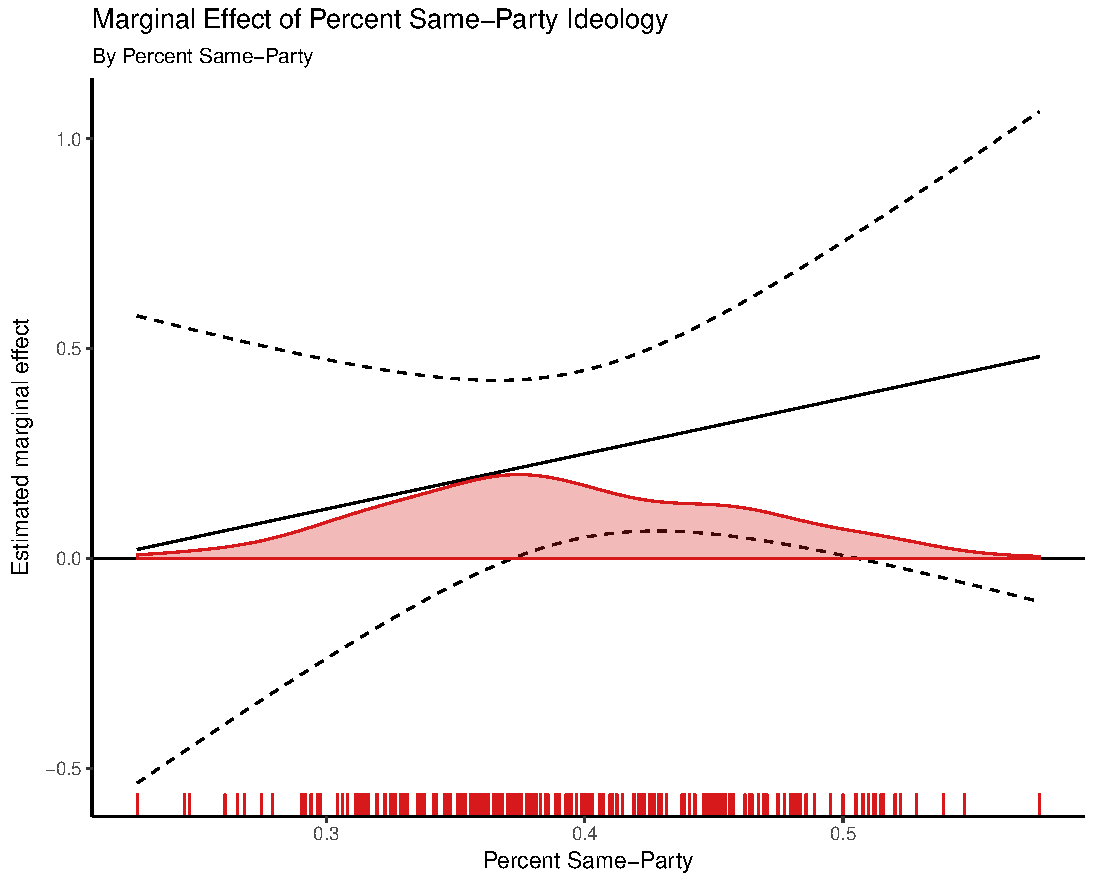
\includegraphics[width=.25\textwidth]{/Users/dsimp/GitHub/Clinton(2006)Rep/drafts/me2-2} &
    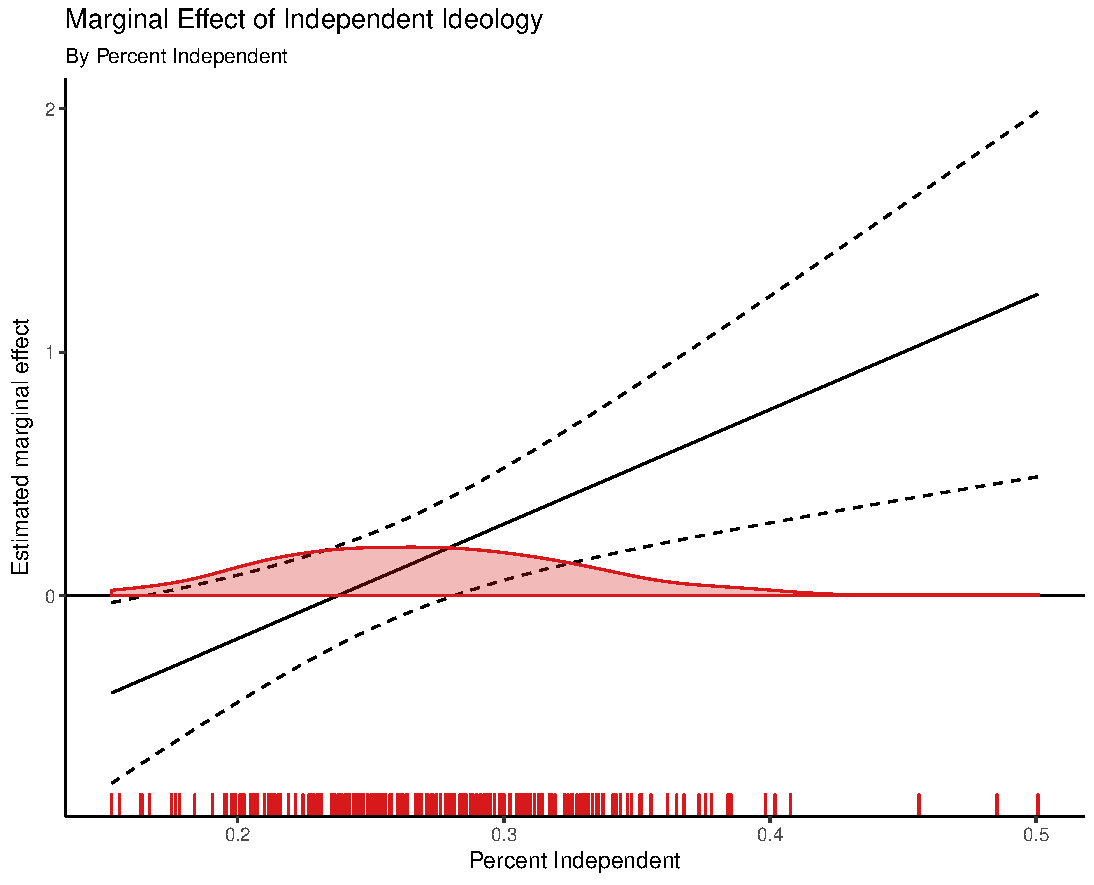
\includegraphics[width=.25\textwidth]{/Users/dsimp/GitHub/Clinton(2006)Rep/drafts/me2-4} &
    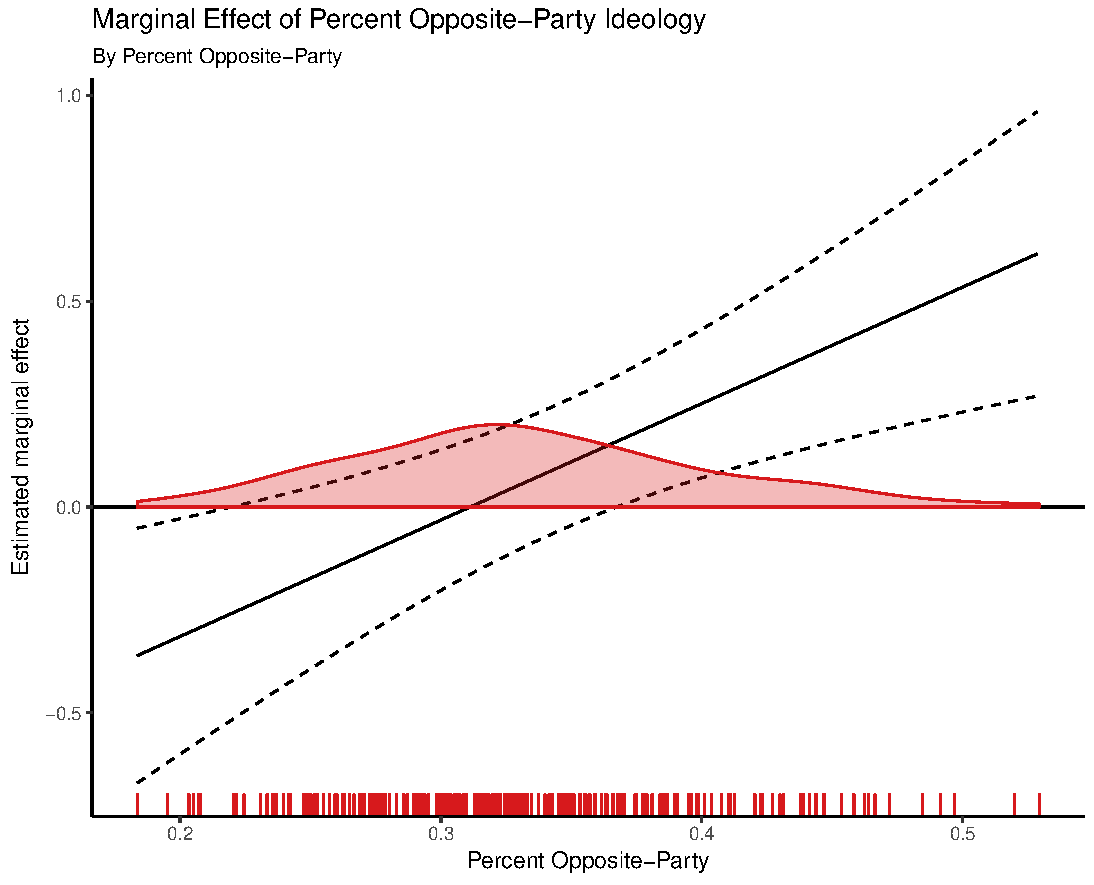
\includegraphics[width=.25\textwidth]{/Users/dsimp/GitHub/Clinton(2006)Rep/drafts/me2-6} \\
    	& & \\ 
	& \small \textbf{DEM Regression} & \\ 
	& & \\ 
  	\small (G) Percent Same-Party& 
  	\small (H) Percent Opposite-Party& 
    \small (I) Percent Independent\\
    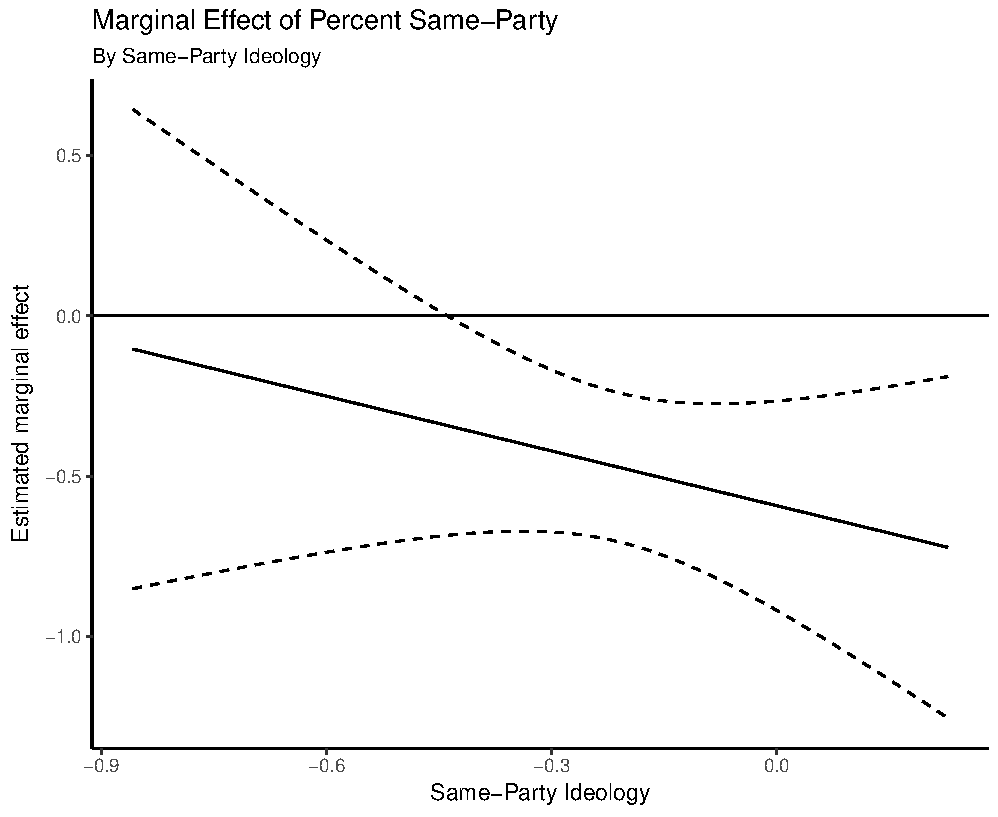
\includegraphics[width=.25\textwidth]{/Users/dsimp/GitHub/Clinton(2006)Rep/drafts/me3-1} &
    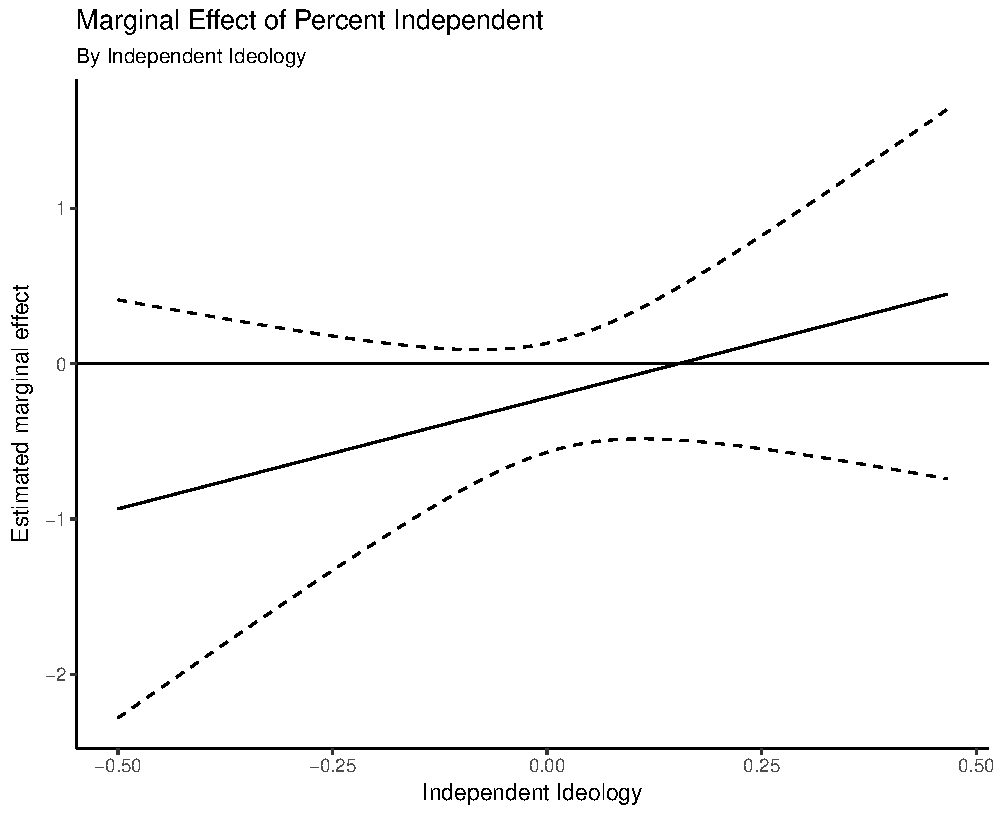
\includegraphics[width=.25\textwidth]{/Users/dsimp/GitHub/Clinton(2006)Rep/drafts/me3-3} &
    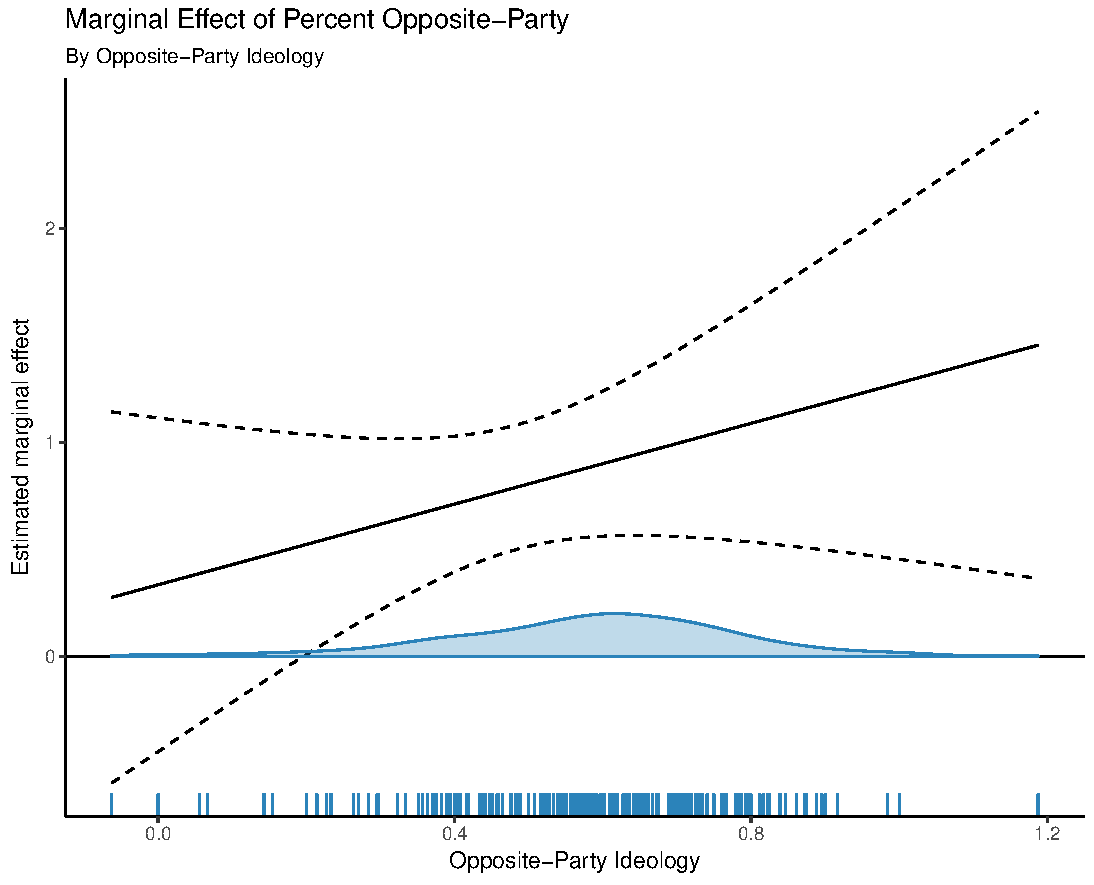
\includegraphics[width=.25\textwidth]{/Users/dsimp/GitHub/Clinton(2006)Rep/drafts/me3-5} \\
     & & \\
  	\small (J) Same-Party Ideology& 
  	\small (K) Opposite-Party Ideology& 
    \small (H) Independent Ideology\\
    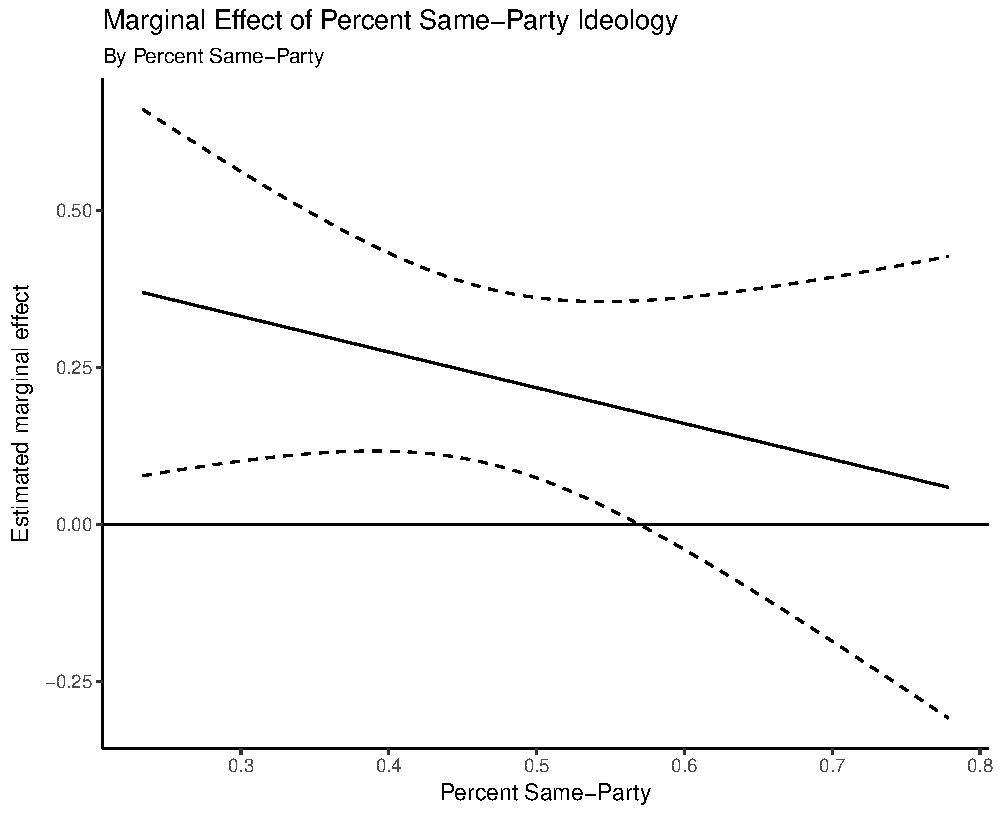
\includegraphics[width=.25\textwidth]{/Users/dsimp/GitHub/Clinton(2006)Rep/drafts/me3-2} &
    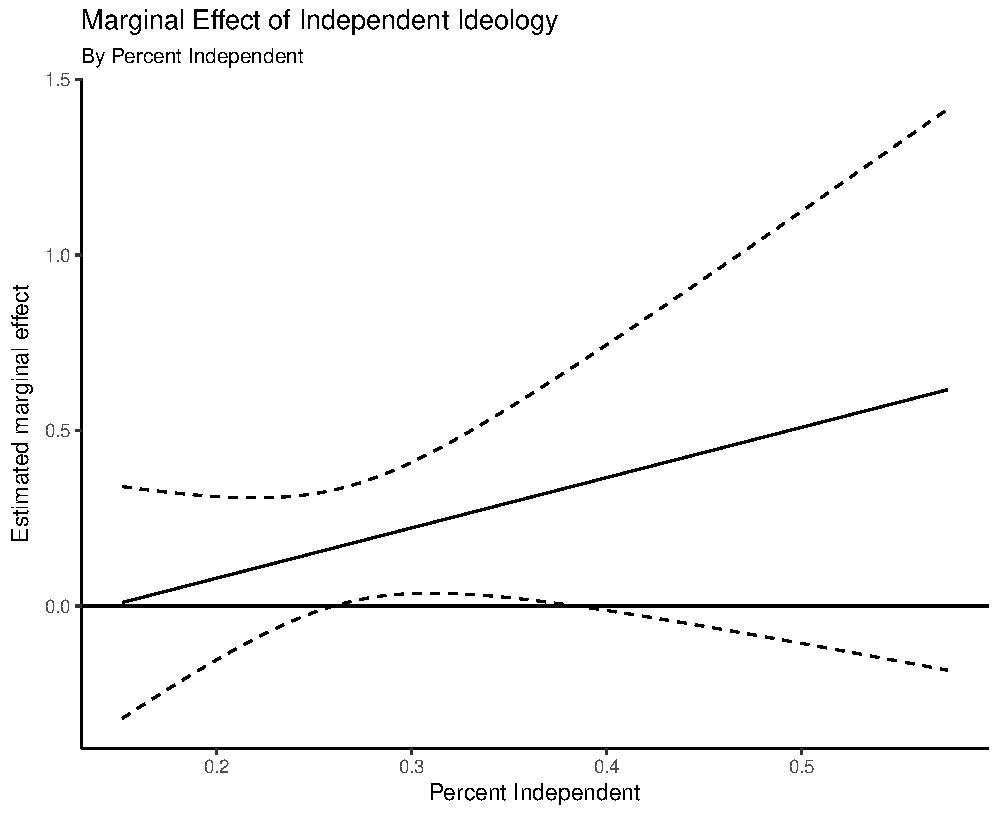
\includegraphics[width=.25\textwidth]{/Users/dsimp/GitHub/Clinton(2006)Rep/drafts/me3-4} &
    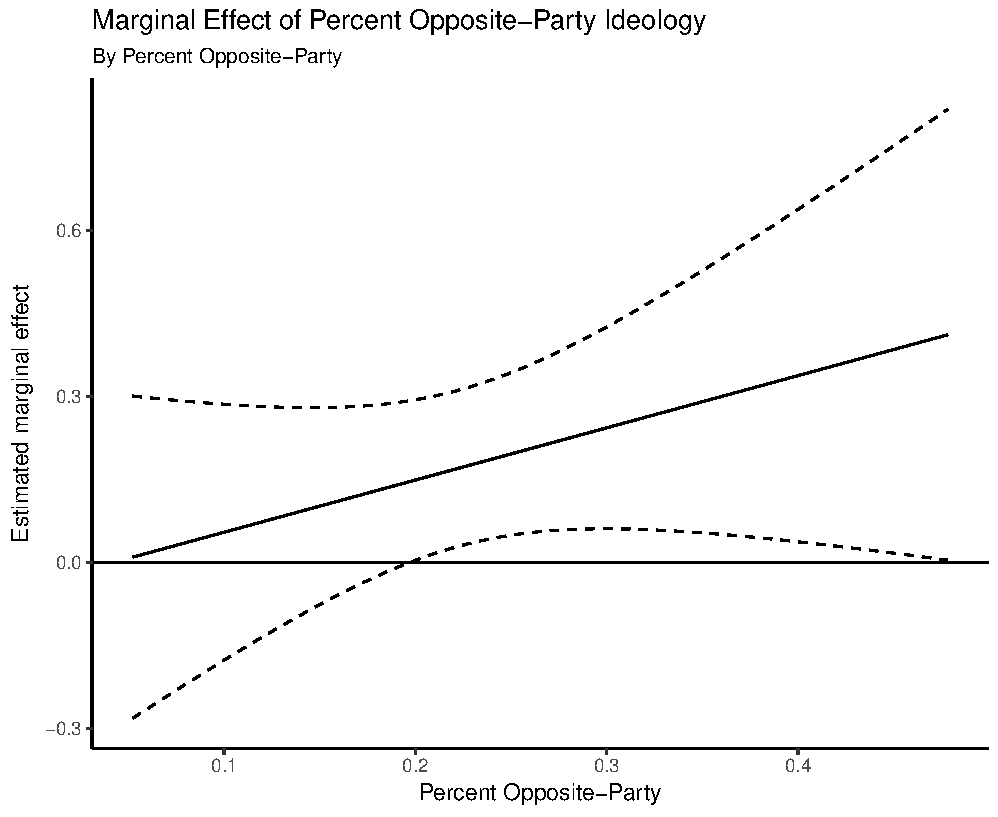
\includegraphics[width=.25\textwidth]{/Users/dsimp/GitHub/Clinton(2006)Rep/drafts/me3-6} \\
     & & \\
  \end{tabular}
    %}   
 \end{centering}\\
  \textbf{Note:} . 
\end{figure}

\newpage

\subsection{Delegate Paradox}
To first explore the Delegate Paradox, I plan to consider the relationship between district ideology and legislator ideal points using all votes in the 106th House and then key votes in the 106th House. Clinton provides both of these measures in the replication data. Observe Table 1, Representative ideal points have a smaller mean and a larger standard deviation when measured using key votes rather than all votes. I then plan to consider the relationship between district ideology and legislator behavior on individual bills using a probit model.

To further explore the Delegate Paradox, I plan to compare the voting behavior of different party legislators with similar district ideologies. I then plan to compare the voting behavior of legislators who won in close elections using election data from the 1998 Midterm election.

Long term, I plan to employ MRP and consider the voting behavior of legislator using survey data related to key votes in the 106th House.

\newpage

\input{/Users/dsimp/GitHub/Clinton(2006)Rep/drafts/table4.txt}


% 

\begin{figure}[!htbp]
\caption{Marginal Effects of Interaction Terms (Key Votes)}
\begin{centering}
%\centering
%\fbox{
  \begin{tabular}{ccc}%{@{}ccc@{}}
	& \small \textbf{GOP Regression} & \\ 
	& & \\ 	
  	\small (A) Percent Same-Party& 
  	\small (B) Percent Opposite-Party& 
    \small (C) Percent Independent\\
    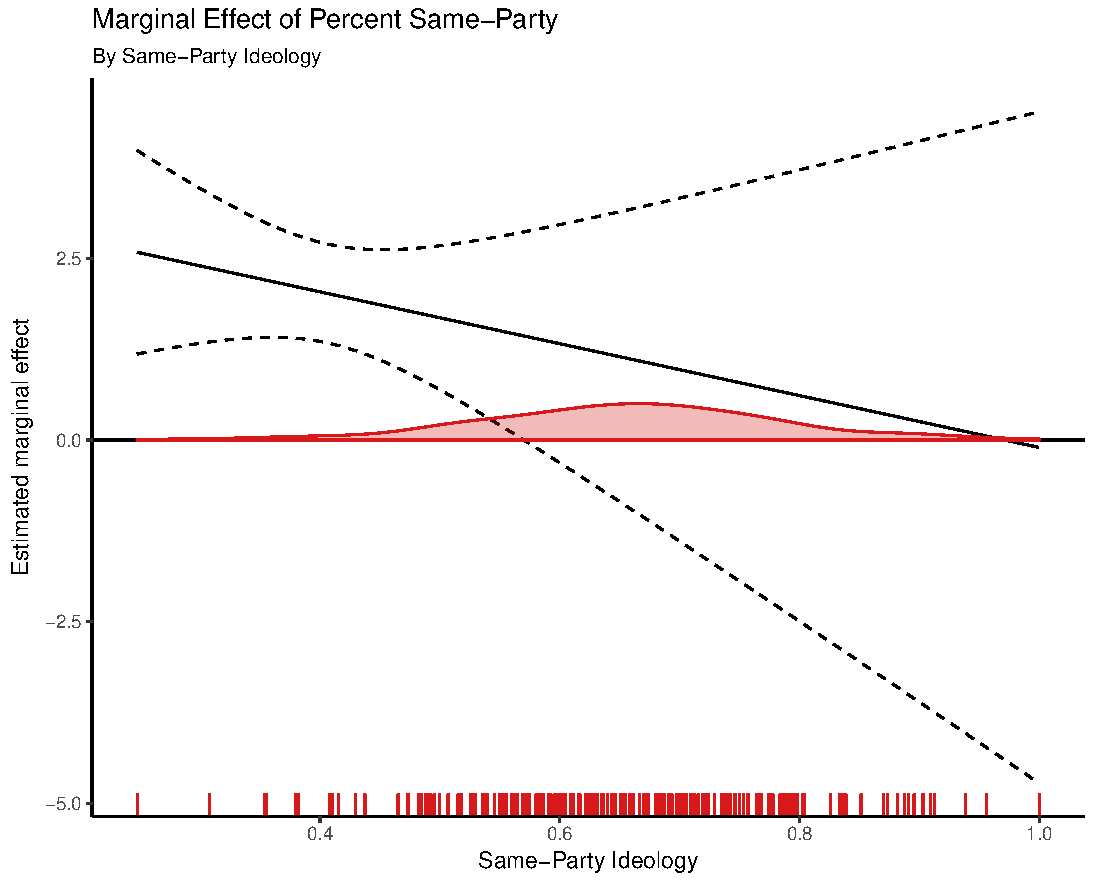
\includegraphics[width=.25\textwidth]{/Users/dsimp/GitHub/Clinton(2006)Rep/drafts/me4-1} &
    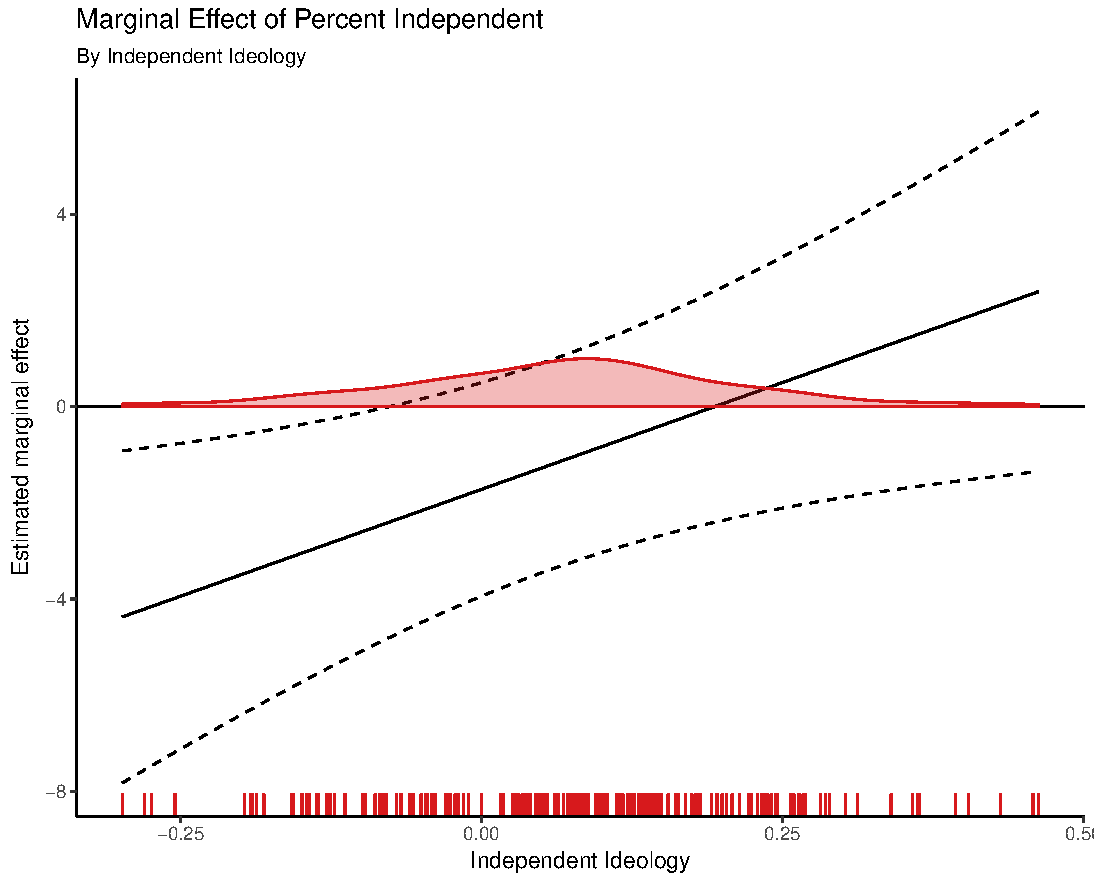
\includegraphics[width=.25\textwidth]{/Users/dsimp/GitHub/Clinton(2006)Rep/drafts/me4-3} &
    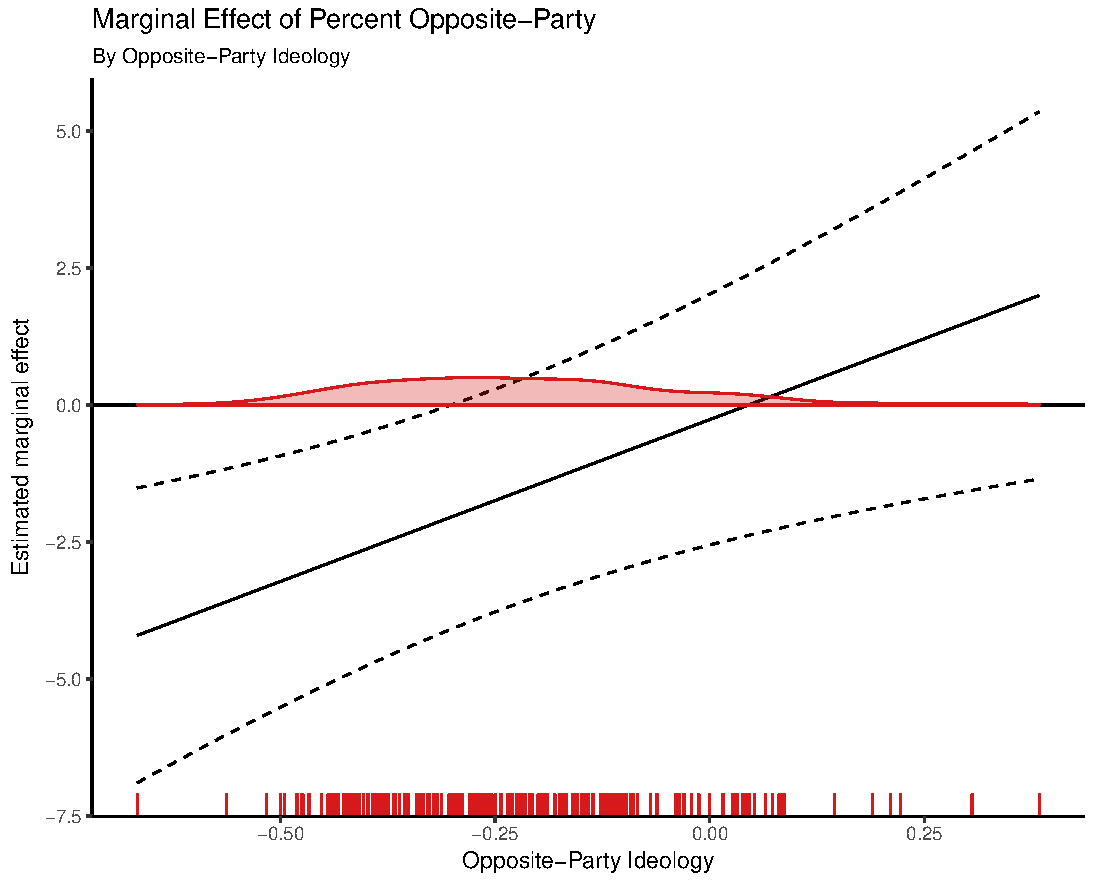
\includegraphics[width=.25\textwidth]{/Users/dsimp/GitHub/Clinton(2006)Rep/drafts/me4-5} \\
     & & \\
  	\small (D) Same-Party Ideology& 
  	\small (E) Opposite-Party Ideology& 
    \small (F) Independent Ideology\\
    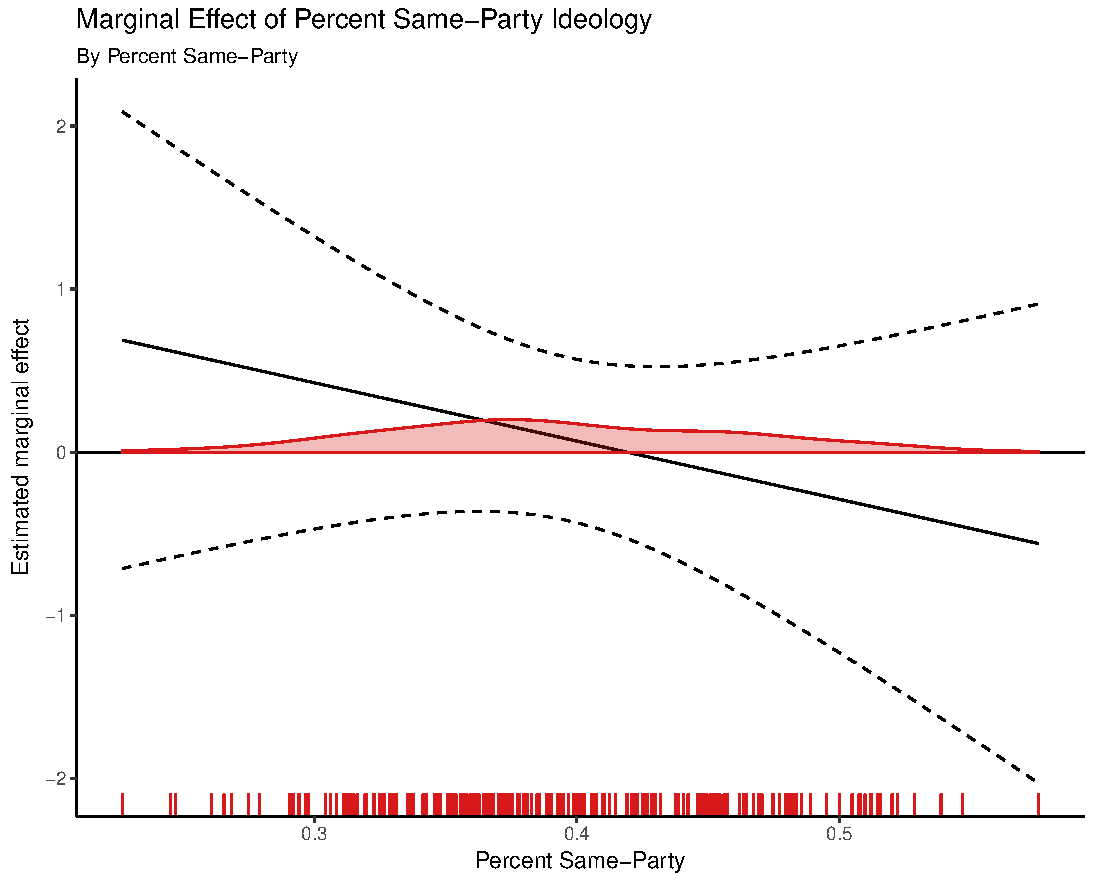
\includegraphics[width=.25\textwidth]{/Users/dsimp/GitHub/Clinton(2006)Rep/drafts/me4-2} &
    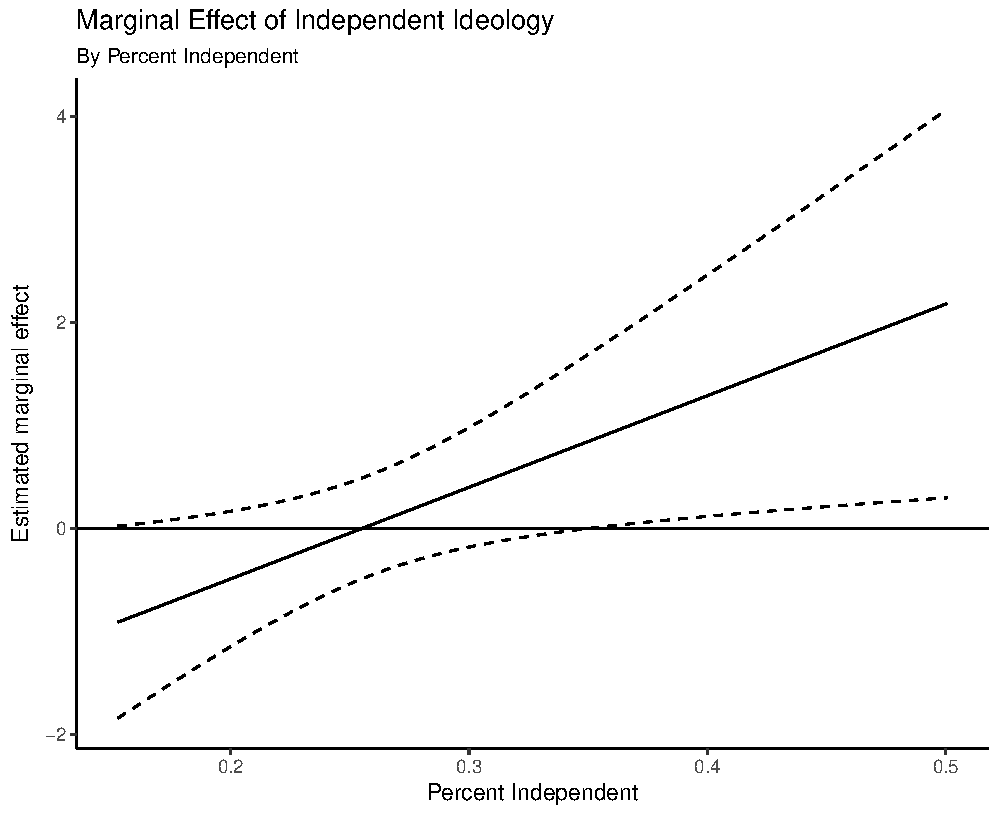
\includegraphics[width=.25\textwidth]{/Users/dsimp/GitHub/Clinton(2006)Rep/drafts/me4-4} &
    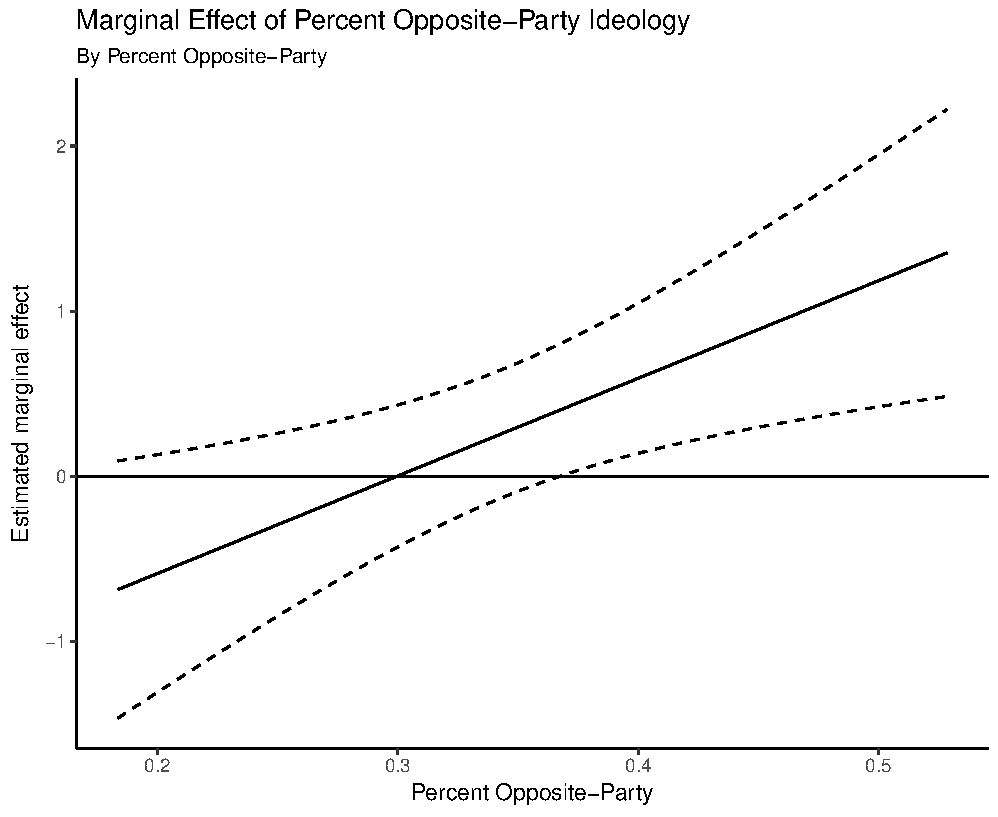
\includegraphics[width=.25\textwidth]{/Users/dsimp/GitHub/Clinton(2006)Rep/drafts/me4-6} \\
    	& & \\ 
	& \small \textbf{DEM Regression} & \\ 
	& & \\ 
  	\small (G) Percent Same-Party& 
  	\small (H) Percent Opposite-Party& 
    \small (I) Percent Independent\\
    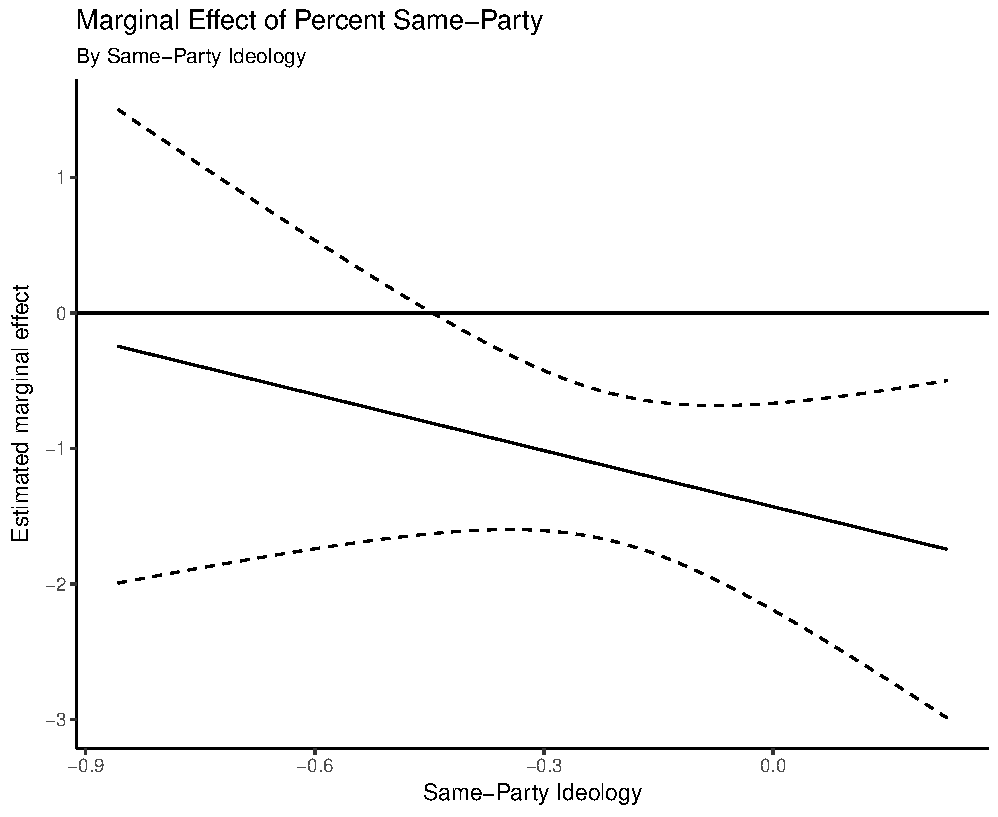
\includegraphics[width=.25\textwidth]{/Users/dsimp/GitHub/Clinton(2006)Rep/drafts/me5-1} &
    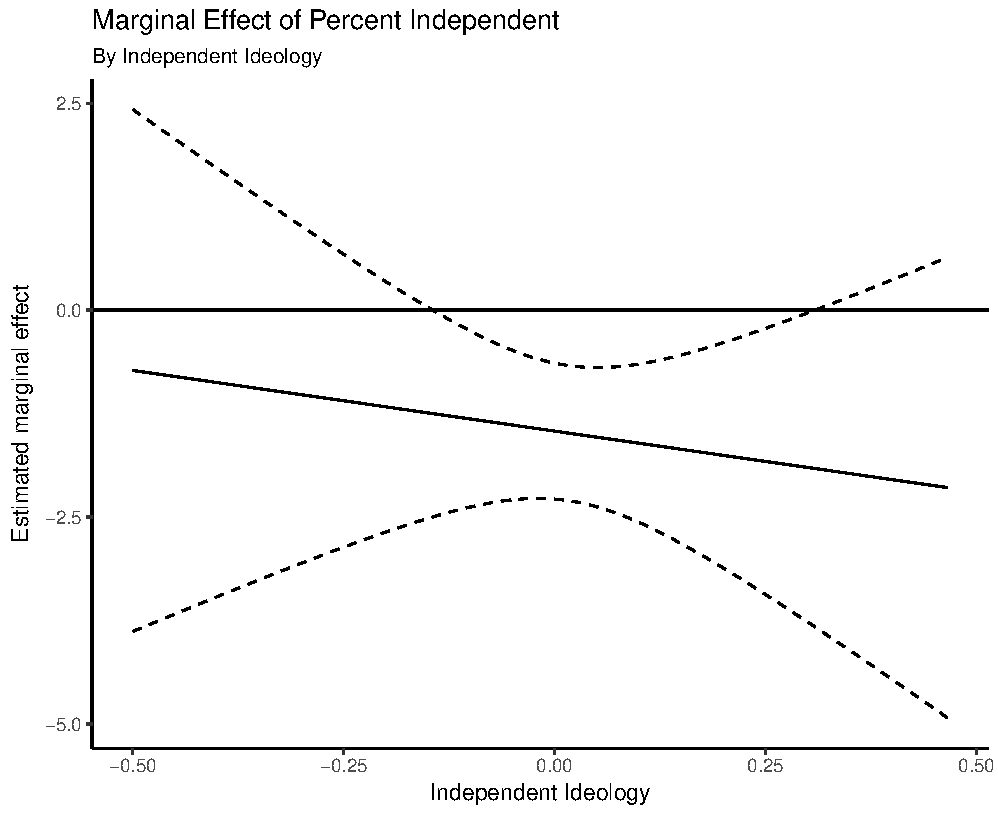
\includegraphics[width=.25\textwidth]{/Users/dsimp/GitHub/Clinton(2006)Rep/drafts/me5-3} &
    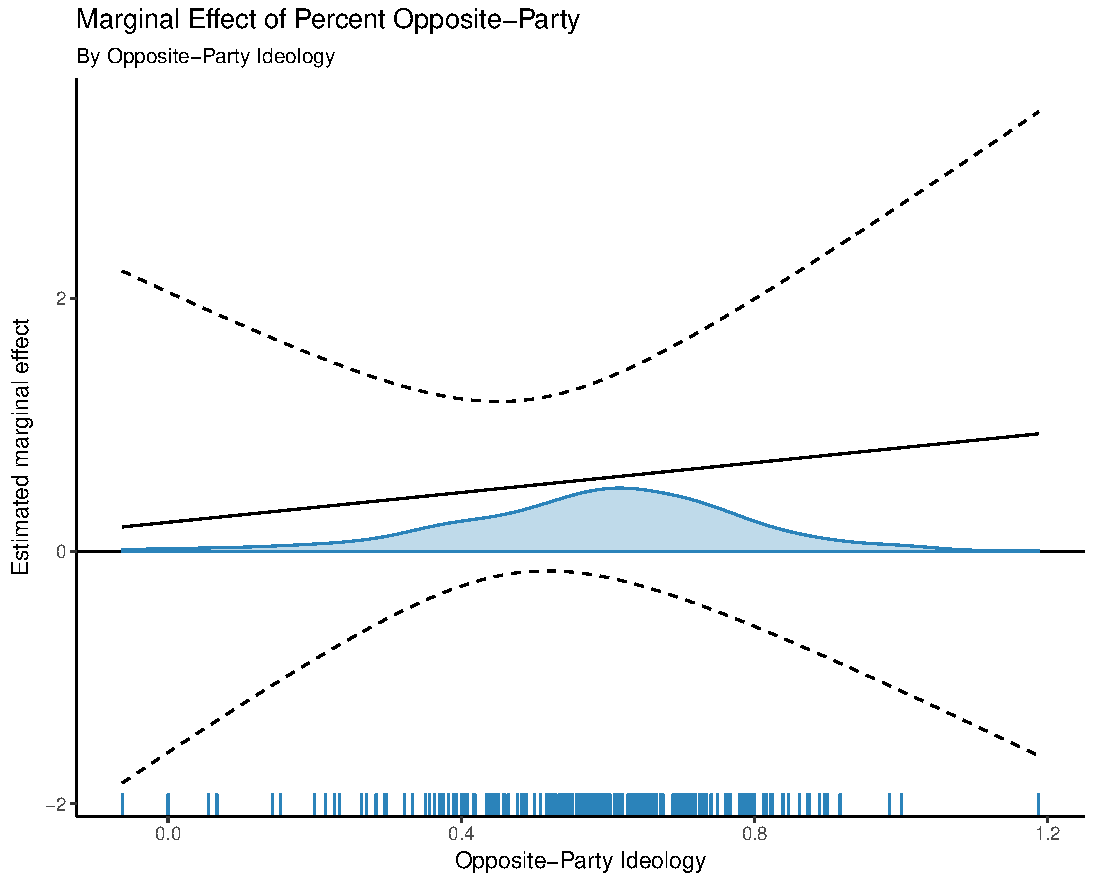
\includegraphics[width=.25\textwidth]{/Users/dsimp/GitHub/Clinton(2006)Rep/drafts/me5-5} \\
     & & \\
  	\small (J) Same-Party Ideology& 
  	\small (K) Opposite-Party Ideology& 
    \small (H) Independent Ideology\\
    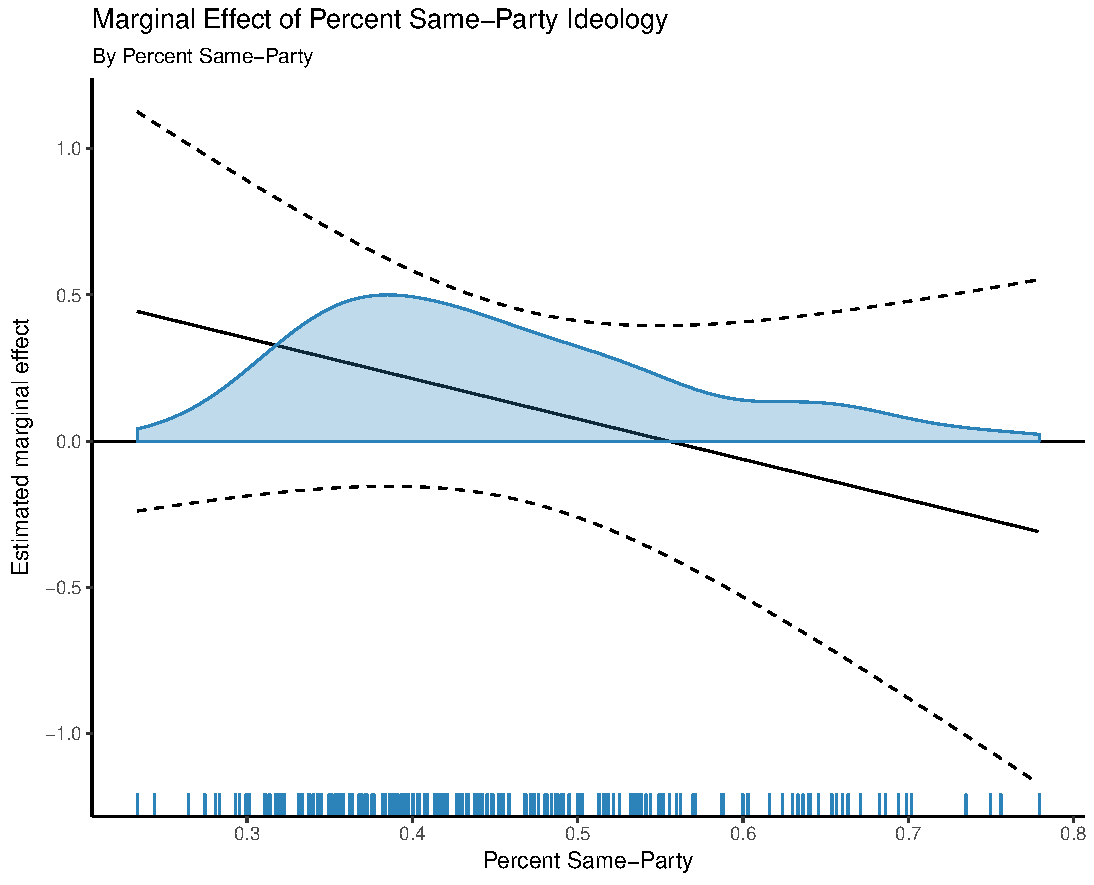
\includegraphics[width=.25\textwidth]{/Users/dsimp/GitHub/Clinton(2006)Rep/drafts/me5-2} &
    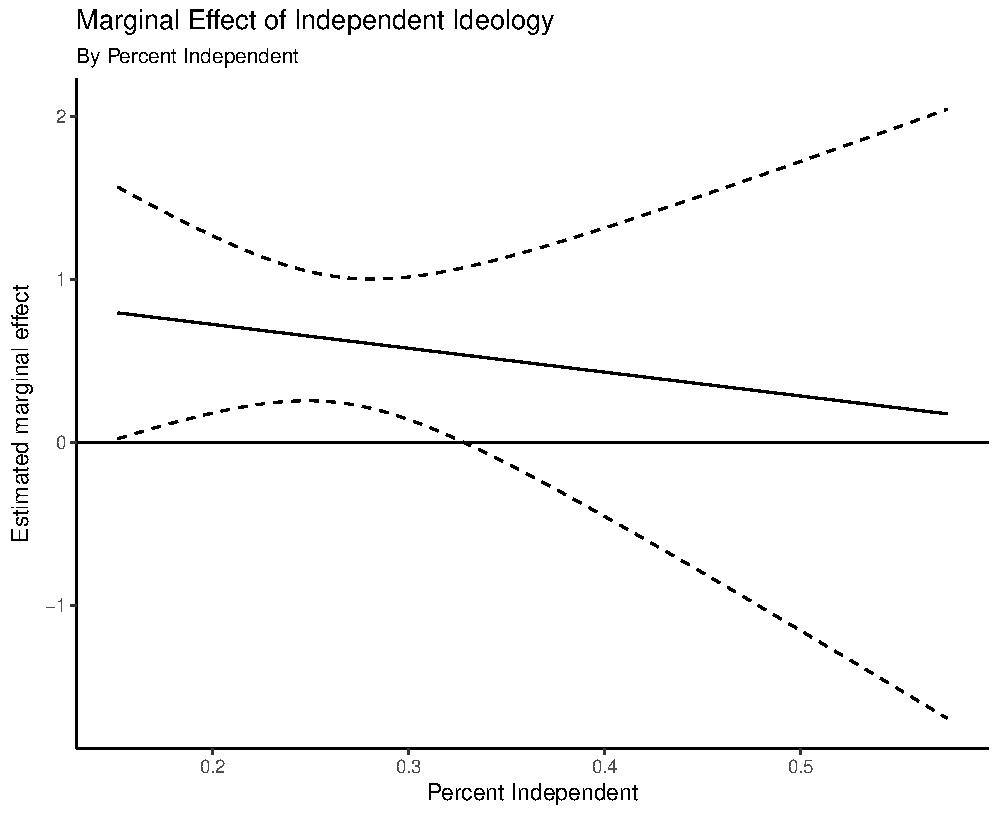
\includegraphics[width=.25\textwidth]{/Users/dsimp/GitHub/Clinton(2006)Rep/drafts/me5-4} &
    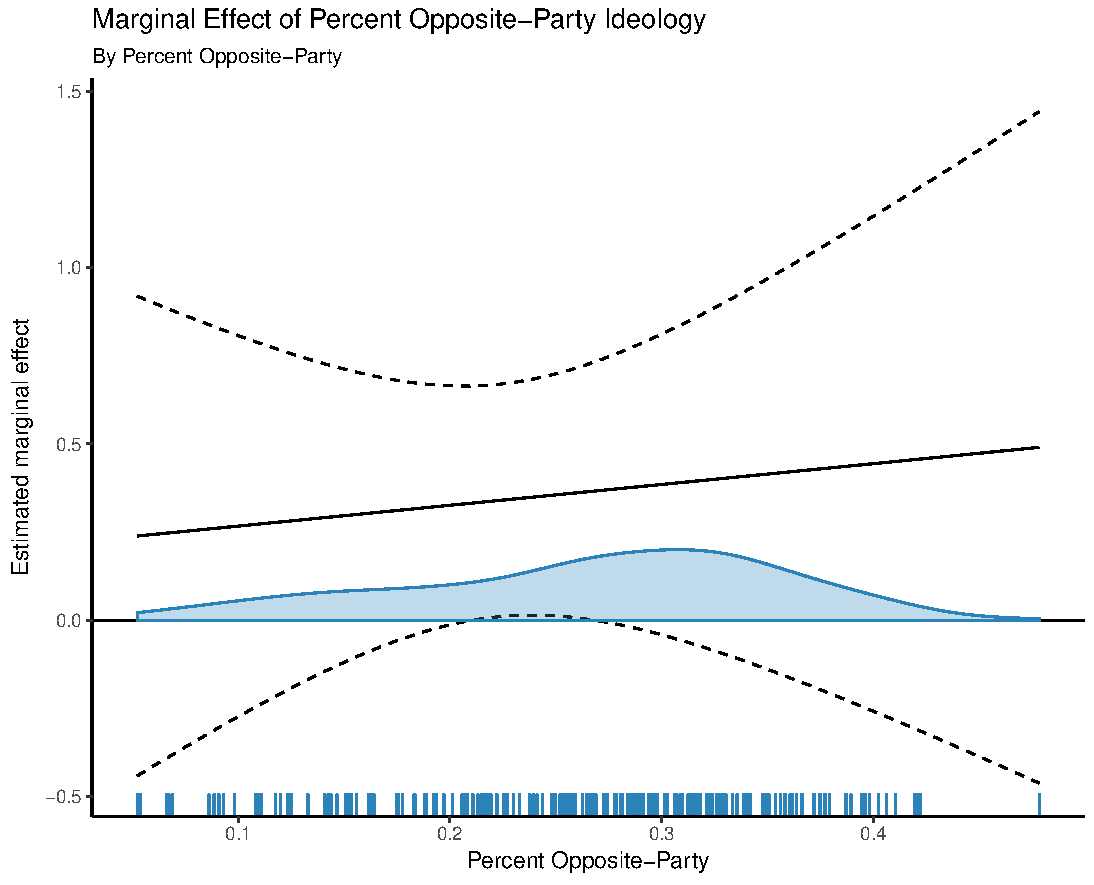
\includegraphics[width=.25\textwidth]{/Users/dsimp/GitHub/Clinton(2006)Rep/drafts/me5-6} \\
     & & \\
  \end{tabular}
    %}   
 \end{centering}\\
  \textbf{Note:} . 
\end{figure}

\newpage


\subsection{Non-Common Scale}
To consider the Non-Common Scales issue I propose running the equation (3) specification using two additional methods for generating ideology scores \textbf{DW-Nominate}, and \textbf{CF-Scores}. Though all three measures are correlated, this procedure will explore how different measures affect the slope between district opinion ideology and legislator ideal points. Furthermore, it will demonstrate why the Non-Common Scale problem implies that the slope and intercept of the responsiveness curve lack direct meanings.The representative ideal points in Clinton (2006) were generated using a methodology described in Clinton (2004).


I have reproduced Clinton (2009) Figure 1. Below it is followed by replication results from Clinton (2009) Table 1 and Table 2. In each table I have reproduced Clinton's OLS findings and also included replication regression where I use Same-Party Ideology, Independent Ideology and Opposite Party Ideology.













\newpage
%\input{/Users/dsimp/GitHub/Clinton(2006)Rep/drafts/table3.txt}

\newpage


\newpage

\newpage


\section{Conclusion} 
This paper has demonstrated that independent voters cannot be lumped with opposite party voters when studying the relationship between legislator voting behavior and sub-district constituent ideology. It also explore the sensitivity of various forms of ideology measures.

Future extensions of this project include comparing the stability of the results with other measures of legislator ideal points as well as to employ MRP for individual topic analysis.

Possible extensions to this project include a more in depth analysis of the Non-Common scale issue. Potential datasets include DW-Nominate Scores as well as CF-Scores. Such analysis would further tease out the consistency of using legislator votes to measure the relationship between behavior and sub-district ideology.

Another extension could consider using survey data. I would plan to identify data relevant to key votes in the 106th House. I would then use MRP to consider the relationship between voter preferences and outcomes on kev votes by topic. This would allow me to compare legislator responsiveness to district ideology to legislator responsiveness to district issue preferences.


A longer term extension of this project would be to 

Election Results data to explore the behavior of legislators who won close elections.
Census data - to explore how legislator ideal points varies with district ideology and district demographic characteristics. 




\begin{sidewaystable}[!htbp] \centering 
  \caption{} 
  \label{} 
\begin{tabular}{@{\extracolsep{5pt}}lccccccc} 
\\[-1.8ex]\hline \\[-1.8ex] 
Statistic & \multicolumn{1}{c}{N} & \multicolumn{1}{c}{Mean} & \multicolumn{1}{c}{St. Dev.} & \multicolumn{1}{c}{Min} & \multicolumn{1}{c}{Pctl(25)} & \multicolumn{1}{c}{Pctl(75)} & \multicolumn{1}{c}{Max} \\ 
\hline \\[-1.8ex] 
Legislator Ideal Pt & 432 & 0.324 & 0.527 & $-$1.000 & $-$0.139 & 0.802 & 1.240 \\ 
Legisaltor Ideal Pt KV & 432 & 0.036 & 0.941 & $-$2.010 & $-$0.752 & 0.818 & 2.110 \\ 
Legislator Ideal Pt Prec & 432 & 45726.000 & 660212.000 & 98.300 & 519.000 & 933.000 & 9736997.000 \\ 
Legislator Ideal Pt KV Prec & 432 & 46029.000 & 675447.000 & 2.540 & 7.510 & 26.900 & 10074884.000 \\ 
District & 432 & 2797.000 & 1571.000 & 101 & 1304.0 & 4102.0 & 5600 \\ 
Party & 432 & 152.000 & 50.700 & 100 & 100 & 200 & 328 \\ 
Mean Ideolgoy & 432 & 0.126 & 0.172 & $-$0.618 & 0.034 & 0.253 & 0.526 \\ 
Mean SP Ideology & 432 & 0.211 & 0.487 & $-$0.858 & $-$0.257 & 0.661 & 1.000 \\ 
Mean NSP Ideology & 432 & 0.098 & 0.244 & $-$0.541 & $-$0.105 & 0.303 & 0.667 \\ 
Mean OP Ideology & 432 & 0.173 & 0.443 & $-$0.667 & $-$0.243 & 0.597 & 1.190 \\ 
Mean IND Ideology & 432 & 0.047 & 0.161 & $-$0.500 & $-$0.048 & 0.140 & 0.467 \\ 
StDev Ideology & 432 & 0.928 & 0.056 & 0.762 & 0.891 & 0.960 & 1.220 \\ 
StDev SP Ideology & 432 & 0.834 & 0.091 & 0.577 & 0.773 & 0.887 & 1.210 \\ 
StDev NSP Ideology & 432 & 0.879 & 0.080 & 0.681 & 0.823 & 0.923 & 1.330 \\ 
StDev OP Ideology & 432 & 0.843 & 0.115 & 0.515 & 0.775 & 0.903 & 1.550 \\ 
StDev IND Ideology & 432 & 0.852 & 0.104 & 0.577 & 0.786 & 0.910 & 1.280 \\ 
Respondents & 432 & 232.000 & 152.000 & 41 & 178 & 254 & 2099 \\ 
SP Respondents & 432 & 86.600 & 44.500 & 15 & 64 & 99.2 & 571 \\ 
NSP Respondents & 432 & 125.000 & 103.000 & 18 & 94 & 140 & 1443 \\ 
IND Respondents & 432 & 61.300 & 68.500 & 8 & 43 & 67 & 984 \\ 
OP Respondents & 432 & 64.100 & 39.500 & 6 & 45 & 76 & 459 \\ 
Avg 2P Pres Vote & 432 & 0.536 & 0.130 & 0.252 & 0.450 & 0.600 & 0.924 \\ 
District SqMi & 432 & 8.030 & 7.390 & $-$1 & 2 & 12 & 43 \\ 
Tenure & 432 & 8727.000 & 34470.000 & 0.000 & 421.000 & 7708.000 & 654334.000 \\ 
\hline \\[-1.8ex] 
\end{tabular} 
\end{sidewaystable} 



\newpage

\newpage

\bibliography{citations}


\end{document}